\documentclass[11pt]{amsbook}
\usepackage[margin=1.1in]{geometry}
\usepackage{amsmath,amssymb,amsthm,mathtools}
\usepackage{graphicx}
\usepackage{booktabs}
\usepackage{enumitem}
\usepackage{tikz-cd}
\usepackage{microtype}
\usepackage[hidelinks]{hyperref}
\usepackage{url}

\graphicspath{{figures/}}
\setcounter{tocdepth}{1}
\numberwithin{equation}{chapter}
\allowdisplaybreaks

\theoremstyle{plain}
\newtheorem{theorem}{Theorem}[chapter]
\newtheorem{proposition}[theorem]{Proposition}
\newtheorem{lemma}[theorem]{Lemma}
\newtheorem{corollary}[theorem]{Corollary}
\newtheorem{maintheorem}{Theorem}
\renewcommand{\themaintheorem}{\Alph{maintheorem}}
\theoremstyle{definition}
\newtheorem{definition}[theorem]{Definition}
\newtheorem{example}[theorem]{Example}
\newtheorem{question}[theorem]{Question}
\theoremstyle{remark}
\newtheorem{remark}[theorem]{Remark}

\newcommand{\R}{\mathbb{R}}
\newcommand{\C}{\mathbb{C}}
\newcommand{\Hq}{\mathbb{H}}
\newcommand{\Oc}{\mathbb{O}}
\newcommand{\K}{\mathbb{K}}
\newcommand{\Z}{\mathbb{Z}}
\newcommand{\Q}{\mathbb{Q}}
\newcommand{\Sp}{\mathrm{Sp}}
\newcommand{\SO}{\mathrm{SO}}
\newcommand{\U}{\mathrm{U}}
\newcommand{\RP}{\mathbb{RP}}
\newcommand{\CP}{\mathbb{CP}}
\newcommand{\KP}{\mathbb{KP}}
\newcommand{\HP}{\mathbb{HP}}
\newcommand{\lk}{\operatorname{lk}}
\newcommand{\Hopf}{\mathrm{H}}
\newcommand{\im}{\operatorname{im}}
\newcommand{\Imag}{\operatorname{Im}}
\renewcommand{\Re}{\operatorname{Re}}

\raggedbottom
\begin{document}

\frontmatter
\title[Homotopy groups of spheres, Hopf fibrations and Villarceau circles II]{Homotopy Groups of Spheres, Hopf Fibrations\\ and Villarceau Circles II}
\author{Deep Bhattacharjee}
\address{Formerly, Electro-Gravitational Space Propulsion Laboratory (EGSPL), Bhubaneswar, Odisha 751030, India}
\address{Formerly, University of Calcutta (Heramba Chandra College), 23/49 Gariahat Road, Golpark, Kolkata 700029, West Bengal, India}
\email{d.bhattacharjee@erl-forschung.de}
\email{itsdeep@live.com}
\email{egspl@proton.me}
\urladdr{https://orcid.org/0000-0003-0466-750X}
\thanks{This is version 2 of the preprint ``Homotopy Groups of Spheres, Hopf Fibrations and Villarceau Circles II'', Preprints.org, 28 February 2026, \texttt{doi:10.20944/preprints202602.2038.v1}, which it revises and replaces. An earlier version of the work appeared as D.~Bhattacharjee, S.~Singha Roy and R.~Sadhu, ``Homotopy group of spheres, Hopf fibrations and Villarceau circles'', EPRA International Journal of Research \& Development (IJRD) \textbf{7} (2022), no.~9, \texttt{doi:10.36713/epra11212}. Corresponding author: Deep Bhattacharjee, \texttt{d.bhattacharjee@erl-forschung.de}; contact for the accompanying repository \url{https://github.com/creelie/Paper_6}: \texttt{egspl@proton.me}.}
\subjclass[2020]{55Q05, 55Q25, 55R10, 53A05}
\keywords{Hopf fibration, Hopf invariant, Villarceau circles, homotopy groups of spheres}
\date{}

\begin{abstract}
We prove that the stereographic images of the fibres of the complex, quaternionic and octonionic Hopf fibrations lying on a product of two round spheres are the Villarceau spheres of a tube, which gives Villarceau's theorem for every ring torus, and that the Hopf invariant of a holomorphic polynomial map $[P:Q]\colon S^3\to S^2$ is the number of common zeros of $P$ and $Q$ in the open four-ball, hence at most $\deg P\cdot\deg Q$. Along the way we give complete proofs that the three Hopf maps are sphere bundles of vector bundles with Hopf invariant one, realise every Hopf invariant by explicit polynomial maps, and derive the homotopy groups of $S^2$, $S^4$ and $S^8$ from those of $S^3$ and $S^7$.
\end{abstract}

\maketitle
\tableofcontents

\mainmatter
\chapter{Introduction}\label{ch:intro}

\section{The objects}

A continuous map between spheres is determined up to homotopy by remarkably little, and yet the groups $\pi_i(S^n)$ of such maps are among the hardest invariants in mathematics to compute. Below the dimension of the target nothing happens: $\pi_i(S^n)=0$ for $i<n$. In the dimension of the target the degree is a complete invariant, $\pi_n(S^n)\cong\Z$. The first surprise is $\pi_3(S^2)\cong\Z$, found by Hopf in 1931 \cite{Hop31}: a map from a three-sphere onto a two-sphere can wrap in infinitely many essentially different ways, and the generator is the map
\begin{equation}\label{eq:intro-hopf}
h\colon S^3\to S^2,\qquad h(z,w)=\bigl(2z\bar w,\;|z|^2-|w|^2\bigr)\in\C\times\R=\R^3 ,
\end{equation}
whose fibres are the great circles $\{(\lambda z,\lambda w):|\lambda|=1\}$. Any two of these circles are linked once. Seen in $\R^3$ through stereographic projection, the fibres lying over a circle of latitude sweep out a torus of revolution, and on that torus they are not meridians, not parallels, but the oblique circles discovered by Yvon Villarceau in 1848 \cite{Vil48}: the circles cut from a ring torus by a plane through its centre that touches it at two points.

Hopf's construction has exactly two more analogues, built from the quaternions and the octonions, with fibres $S^3$ and $S^7$ \cite{Hop35}. Adams' theorem on the Hopf invariant \cite{Ada60} says that there are no others, and that no sphere bundle $S^{d-1}\to S^{2d-1}\to S^d$ exists unless $d\in\{1,2,4,8\}$.

This monograph gives a complete account of these objects with proofs, and it adds results that make the connection between homotopy and geometry precise. We have aimed at a text in which every statement is either proved here or is a published theorem quoted with its source; the deep inputs that are quoted, and not reproved, are listed in Section~\ref{sec:inputs}. Nothing below depends on a conjecture. The text replaces the earlier versions \cite{BSS22}, \cite{Bha26a} of this work, which were expository, corrects their errors, and adds Theorems~\ref{thm:D} and \ref{thm:E}, Proposition~\ref{prop:twofamilies} and the results of Chapter~\ref{ch:villarceau} on Villarceau spheres.

\section{Results}

Throughout, $\K$ is one of the four normed division algebras $\R,\C,\Hq,\Oc$ and $d=\dim_\R\K\in\{1,2,4,8\}$. We write $\bar x$ for the conjugate of $x\in\K$ and $|x|^2=x\bar x$. The \emph{Hopf map} of $\K$ is
\begin{equation}\label{eq:intro-hk}
h_\K\colon S^{2d-1}\to S^d,\qquad h_\K(a,b)=\bigl(2a\bar b,\;|a|^2-|b|^2\bigr)\in\K\times\R=\R^{d+1},
\end{equation}
where $S^{2d-1}$ is the unit sphere of $\K^2=\R^{2d}$. For $x\in\K$ let
\[
L_x=\{(xc,c):c\in\K\}\subset\K^2,\qquad L_\infty=\K\times\{0\}.
\]
These are real linear subspaces of dimension $d$, and we view the family $\{L_x\}$ as parametrised by the one-point compactification $\K\cup\{\infty\}\cong S^d$.

\begin{maintheorem}[Hopf bundles]\label{thm:A}
For each $\K$ the subspaces $L_x$, $x\in\K\cup\{\infty\}$, form a smooth real vector bundle $L_\K$ of rank $d$ over $S^d$, a subbundle of the trivial bundle $S^d\times\K^2$. Every nonzero vector of $\K^2$ lies in exactly one $L_x$, so the unit sphere bundle of $L_\K$ is $S^{2d-1}$ itself, and its projection is the Hopf map \eqref{eq:intro-hk}. The fibres of $h_\K$ are great $(d-1)$-spheres, and the bundle is obtained by gluing two trivial bundles over the hemispheres along the map $x\mapsto(c\mapsto xc)$ of the equator $S^{d-1}$ into $\mathrm{GL}_d(\R)$.
\end{maintheorem}

For $\K=\Oc$ the octonions are not associative, and the usual definition of the octonionic projective line requires care; Theorem~\ref{thm:A} replaces it by an explicit vector bundle. The proof uses only Artin's theorem that two octonions generate an associative subalgebra.

\begin{maintheorem}[Hopf invariant]\label{thm:B}
Let $d\in\{2,4,8\}$.
\begin{enumerate}[label=\textup{(\roman*)}]
\item The Hopf invariant of $h_\K$ is $\pm1$.
\item For every integer $m\ge1$ the power map $x\mapsto x^m$ of the unit sphere $S^{d-1}\subset\K$ has degree $m$, and the map $g_m(a,b)=(a^m,b)/|(a^m,b)|$ of $S^{2d-1}$ has degree $m$.
\item The composite $h_\K\circ g_m$ represents $m[h_\K]$ and has Hopf invariant $\pm m$; composing with $(a,b)\mapsto(\bar a,b)$ gives $-m$. In particular $\Hopf\colon\pi_{2d-1}(S^d)\to\Z$ is onto, and each value is attained by a map whose coordinates are polynomials in the real coordinates of $\K^2$ divided by a norm.
\end{enumerate}
\end{maintheorem}

\begin{maintheorem}[Splitting]\label{thm:C}
For $d\in\{2,4,8\}$ and every $i\ge2$,
\[
\pi_i(S^d)\;\cong\;\pi_i(S^{2d-1})\oplus\pi_{i-1}(S^{d-1}),
\]
where the first summand is embedded by $(h_\K)_*$. In particular $\pi_i(S^2)\cong\pi_i(S^3)$ for $i\ge3$, $\pi_7(S^4)\cong\Z\oplus\Z/12$ and $\pi_{15}(S^8)\cong\Z\oplus\Z/120$, with the infinite cyclic summands generated by the Hopf maps and detected by the Hopf invariant.
\end{maintheorem}

The splitting determines the columns $n=2,4,8$ of the table of $\pi_{n+k}(S^n)$ from the columns $n=3,7$ and from $\pi_*(S^{15})$; Figure~\ref{fig:table} and Table~\ref{tab:unstable} show which entries are derived in this way.

The next result concerns maps $S^3\to S^2$ given by polynomials. For $P,Q\in\C[z,w]$ without common zero on $S^3$ put
\[
[P:Q]\colon S^3\to S^2,\qquad [P:Q](u)=h\bigl(P(u),Q(u)\bigr)\big/\bigl(|P(u)|^2+|Q(u)|^2\bigr),
\]
that is, the point $[P(u):Q(u)]$ of $\CP^1=S^2$.

\begin{maintheorem}[Holomorphic maps]\label{thm:D}
Let $P,Q\in\C[z,w]$ have no common zero on $S^3$, and orient so that $\Hopf(h)=1$. Then $P$ and $Q$ have finitely many common zeros in the open unit ball $B^4\subset\C^2$, and
\[
\Hopf\bigl([P:Q]\bigr)=\sum_{u\in B^4,\ P(u)=Q(u)=0} I_u(P,Q)\;\in\;\bigl[0,\ \deg P\cdot\deg Q\bigr],
\]
where $I_u(P,Q)=\dim_\C\mathcal O_u/(P,Q)$ is the intersection multiplicity. Both bounds are attained, the upper one by $[z^p:w^q]$, whose fibres are torus links of type $(p,q)$ linked $pq$ times. A holomorphic map $[P:Q]$ is null-homotopic exactly when $P$ and $Q$ have no common zero in $B^4$, and every class in $\pi_3(S^2)\cong\Z$ is represented by a map $[P:Q]$ or by its composite with complex conjugation.
\end{maintheorem}

Theorem~\ref{thm:D} turns the Hopf invariant, a homotopy invariant, into an algebraic count, and turns the linking of fibres into an intersection number of plane curves inside the ball.

The last two results are geometric. Let $0<a<1$ and $b=\sqrt{1-a^2}$, and let $\varepsilon\in\K$ be a unit with $\varepsilon\perp1$. Stereographic projection from $N=(0,\varepsilon)$ identifies $S^{2d-1}\setminus\{N\}$ with $\K\times\varepsilon^\perp=\R^d\times\R^{d-1}$.

\begin{maintheorem}[Villarceau spheres]\label{thm:E}
Let $d\in\{2,4,8\}$ and put $R=1/a$, $r=b/a$, so that $R^2-r^2=1$. Stereographic projection maps the product $S^{d-1}(a)\times S^{d-1}(b)$ onto the tube
\[
T_{R,r}=\bigl\{(x,y)\in\R^d\times\R^{d-1}:(|x|-R)^2+|y|^2=r^2\bigr\}
\]
of radius $r$ about the round sphere of radius $R$ in $\R^d\times0$. It maps every fibre of $h_\K$ contained in $S^{d-1}(a)\times S^{d-1}(b)$ onto a round $(d-1)$-sphere of radius $R$, centred at a point at distance $r$ from the origin and lying in a $d$-dimensional linear subspace; these spheres partition $T_{R,r}$. For $d=2$ the tube is a ring torus with $R^2-r^2=1$, the images of the fibres of $h$ form one family of Villarceau circles, and the images of the fibres of $(z,w)\mapsto h(\bar z,w)$ form the other.
\end{maintheorem}

\begin{corollary}[Villarceau's theorem]\label{cor:intro-villarceau}
Let $T$ be a ring torus with radii $R>r>0$. Every plane through the centre of $T$ tangent to $T$ at two points meets $T$ in two circles of radius $R$, and each of the two families of such circles is the image of a family of Hopf fibres under stereographic projection followed by the similarity of ratio $\sqrt{R^2-r^2}$.
\end{corollary}

\begin{maintheorem}[Metric structure]\label{thm:F}
For $\K=\C,\Hq,\Oc$ the Hopf map is a Riemannian submersion from the unit sphere $S^{2d-1}$ onto the sphere $S^d(\tfrac12)$ of radius $\tfrac12$. The fibres are parallel great spheres: the distance between the fibres over $p,q\in S^d$ is half the angle between $p$ and $q$. For $\K=\C$ the fibres over a circle of latitude form a flat torus $S^1(a)\times S^1(b)$ on which they are the closed geodesics of slope $b/a$, and the unit tangent bundle of $S^2$ is the quotient of the Hopf bundle by $\pm1$, a circle bundle over $S^2$ with total space $\RP^3$.
\end{maintheorem}

Chapters~\ref{ch:stable} and \ref{ch:cy} place these results in their wider setting: the stable stems through dimension $19$, the image of the $J$-homomorphism and its Bernoulli denominators, the Kervaire invariant problem, and the torus fibrations of the Strominger--Yau--Zaslow picture, of which the Clifford tori of the Hopf fibration are the simplest example. We state precisely what is known there, prove what is elementary, and separate both from the conjectural.

\section{Inputs taken from the literature}\label{sec:inputs}

The following theorems are used without proof. Each is a published result with a complete proof in the cited source.
\begin{enumerate}[label=(I\arabic*)]
\item Cellular approximation, the long exact sequence of a fibration, the Hurewicz theorem and the Freudenthal suspension theorem \cite[Chapter~4]{Hat02}.
\item Poincar\'e duality for closed oriented manifolds \cite[Section~3.3]{Hat02}.
\item Artin's theorem: the subalgebra of $\Oc$ generated by any two elements is associative \cite[Chapter~III]{Sch66}, \cite{Bae02}.
\item Adams' theorem: an element of Hopf invariant one in $\pi_{2n-1}(S^n)$ exists only for $n=1,2,4,8$ \cite{Ada60}, \cite{AA66}.
\item The degree of the boundary map of a vector field with isolated zeros equals the sum of their indices \cite[Section~6]{Mil65}; the index of an isolated zero of a holomorphic map germ $(\C^2,u)\to(\C^2,0)$ is its intersection multiplicity \cite[Chapter~5]{GH78}, \cite[Chapter~5]{AGV85}; B\'ezout's theorem \cite[Chapter~5]{Ful69}; an irreducible complex algebraic curve is connected in the classical topology \cite[Corollary~(4.16)]{Mum76}.
\item The values of $\pi_{n+k}(S^n)$ for $k\le 7$ and of the stable stems for $k\le19$ \cite{Tod62}, \cite{Rav86}, \cite{IWX23}; the image of $J$ \cite{Ada66}, \cite{Qui71}, \cite{Sul74}, \cite{BG75}; the Kervaire invariant results \cite{Bro69}, \cite{HHR16}.
\item Hopf's description of the Hopf invariant of a map $S^3\to S^2$ as the linking number of two fibres \cite{Hop31}, \cite[Section~17]{BT82}.
\end{enumerate}
Items (I4) and (I6) are deep, and their proofs are not reproduced. The rest of the text is self-contained modulo standard algebraic topology.

\section{Plan}

Chapter~\ref{ch:foundations} fixes conventions and proves the elementary facts about homotopy groups of spheres that are needed, together with a splitting lemma for fibrations whose fibre inclusion is null-homotopic. Chapter~\ref{ch:hopf} constructs the Hopf bundles and proves Theorem~\ref{thm:A}. Chapter~\ref{ch:invariant} treats the Hopf invariant and proves Theorem~\ref{thm:B}; Chapter~\ref{ch:groups} proves Theorem~\ref{thm:C} and derives the table of unstable groups. Chapter~\ref{ch:linking} is about linking numbers and proves Theorem~\ref{thm:D}, together with its analogue for split quaternionic and octonionic maps (Proposition~\ref{prop:split}). Chapter~\ref{ch:geometry} proves Theorem~\ref{thm:F}, and Chapter~\ref{ch:villarceau} proves Theorem~\ref{thm:E} and Villarceau's theorem. The appendices collect the octonion identities, the algebra behind Villarceau's theorem, the tables of stable stems and the numerical checks.

\section{Conventions}

Spheres are $S^n=\{x\in\R^{n+1}:|x|=1\}$ and $S^n(\rho)$ is the sphere of radius $\rho$. Homotopy groups are based, and we drop basepoints from the notation when the space is path connected. A map $f\colon S^n\to S^n$ has a degree $\deg f\in\Z$, defined by $f_*[S^n]=(\deg f)[S^n]$ in $H_n(S^n;\Z)$. We write $\Z/m$ for the cyclic group of order $m$, and in tables a cyclic group is denoted by its order. The words \emph{fibration} and \emph{fibre bundle} are used in their standard senses \cite[Section~4.2]{Hat02}; all fibre bundles below are locally trivial over spheres and therefore Hurewicz fibrations.

\chapter{Homotopy groups and fibrations}\label{ch:foundations}

This chapter collects the facts from homotopy theory used later. Most are standard; we give proofs where the argument is short or where the precise form matters, and we prove one splitting lemma, Lemma~\ref{lem:split}, on which Chapter~\ref{ch:groups} rests.

\section{Homotopy groups}

Let $X$ be a space with basepoint $x_0$. For $i\ge1$ the group $\pi_i(X,x_0)$ is the set of homotopy classes of maps $f\colon(I^i,\partial I^i)\to(X,x_0)$, the homotopies being through maps of the same kind, with the product
\[
(f+g)(t_1,\dots,t_i)=\begin{cases}f(2t_1,t_2,\dots,t_i),&t_1\le\tfrac12,\\ g(2t_1-1,t_2,\dots,t_i),&t_1\ge\tfrac12.\end{cases}
\]
It is abelian for $i\ge2$.\footnote{The two halves of the cube can be shrunk and slid around one another in the second coordinate; for $i=1$ there is no second coordinate, and $\pi_1$ need not be abelian.} Collapsing $\partial I^i$ identifies $\pi_i(X,x_0)$ with the set of based homotopy classes of based maps $(S^i,s_0)\to(X,x_0)$. For a pair $(X,A)$ with $x_0\in A$ and $i\ge1$, the relative set $\pi_i(X,A,x_0)$ consists of homotopy classes of maps $(D^i,S^{i-1},s_0)\to(X,A,x_0)$; it is a group for $i\ge2$, and there is an exact sequence
\begin{equation}\label{eq:pair-les}
\cdots\to\pi_i(A)\to\pi_i(X)\to\pi_i(X,A)\xrightarrow{\ \partial\ }\pi_{i-1}(A)\to\cdots\to\pi_0(X),
\end{equation}
in which $\partial$ restricts a map of $D^i$ to its boundary \cite[Theorem~4.3]{Hat02}.

A \emph{CW complex} is a space $X$ with a filtration $X^0\subset X^1\subset\cdots$ by skeleta, where $X^0$ is discrete and $X^n$ is obtained from $X^{n-1}$ by attaching $n$-cells along maps $S^{n-1}\to X^{n-1}$, and $X=\bigcup_nX^n$ has the weak topology. The closure of each cell then meets only finitely many cells.\footnote{This is the ``closure-finite'' condition that gives CW complexes the letter C. It concerns the closure of a cell, which lies in a finite subcomplex; a cell may well meet the closures of infinitely many others.} The sphere $S^n$ has a CW structure with one $0$-cell $s_0$ and one $n$-cell attached by the constant map. A map $f\colon X\to Y$ of CW complexes is \emph{cellular} if $f(X^n)\subset Y^n$ for all $n$.

\begin{theorem}[Cellular approximation {\cite[Theorem~4.8]{Hat02}}]\label{thm:cellular}
Every map of CW complexes is homotopic to a cellular map, by a homotopy that is stationary on any subcomplex on which the map is already cellular.
\end{theorem}

\begin{proposition}\label{prop:below}
$\pi_i(S^n)=0$ for $0\le i<n$.
\end{proposition}

\begin{proof}
Give $S^i$ and $S^n$ the CW structures with one $0$-cell each, at the basepoints. A based map $f\colon S^i\to S^n$ is cellular on the subcomplex $\{s_0\}$, so by Theorem~\ref{thm:cellular} it is homotopic relative to $s_0$ to a cellular map. A cellular map sends $S^i=(S^i)^i$ into the $i$-skeleton of $S^n$, which is the point $s_0$ because $i<n$. So $f$ is null-homotopic relative to the basepoint.
\end{proof}

\begin{proposition}\label{prop:degree}
For $n\ge1$ the degree defines an isomorphism $\pi_n(S^n)\to\Z$ that sends the identity to $1$. Two maps $S^n\to S^n$ are freely homotopic if and only if they have the same degree.
\end{proposition}

\begin{proof}
For $n=1$ this is the computation of $\pi_1(S^1)$ by covering space theory. For $n\ge2$ the sphere is $(n-1)$-connected by Proposition~\ref{prop:below}, and the Hurewicz homomorphism $\pi_n(S^n)\to H_n(S^n;\Z)\cong\Z$, which sends $[f]$ to $f_*[S^n]=(\deg f)[S^n]$, is an isomorphism \cite[Theorem~4.32]{Hat02}. For the second statement note that $\pi_1(S^n)$ acts trivially on $\pi_n(S^n)$ (for $n\ge2$ it is the trivial group, and for $n=1$ the group is abelian), so free homotopy classes of maps $S^n\to S^n$ coincide with based ones \cite[Section~4.A]{Hat02}.
\end{proof}

The antipodal map of $S^n$ is the composite of $n+1$ reflections, each of degree $-1$, so it has degree $(-1)^{n+1}$.

\begin{lemma}\label{lem:precompose}
Let $X$ be a space, $i\ge1$, $\alpha\in\pi_i(X)$, and let $g\colon S^i\to S^i$ be a based map of degree $m$. Then $\alpha\circ g=m\alpha$.
\end{lemma}

\begin{proof}
For a fixed map $f\colon S^i\to X$, composition $[g]\mapsto[f\circ g]$ is a homomorphism $f_*\colon\pi_i(S^i)\to\pi_i(X)$, because the sum in $\pi_i$ is formed in the source coordinate. By Proposition~\ref{prop:degree} the class of $g$ is $m[\mathrm{id}]$, so $[f\circ g]=f_*(m[\mathrm{id}])=m[f]$.
\end{proof}

\section{Fibrations and the long exact sequence}

A map $p\colon E\to B$ has the \emph{homotopy lifting property} for a space $Y$ if for every homotopy $F\colon Y\times I\to B$ and every lift $\tilde F_0\colon Y\to E$ of $F_0$ there is a homotopy $\tilde F$ lifting $F$ and starting at $\tilde F_0$. It is a \emph{Serre fibration} if it has this property for all cubes $Y=I^k$, and a \emph{Hurewicz fibration} if it has it for all spaces. Every fibre bundle is a Serre fibration, and a fibre bundle over a paracompact base is a Hurewicz fibration \cite[Proposition~4.48 and the remarks after it]{Hat02}.\footnote{Covering spaces are fibre bundles with discrete fibre; for them the lift is unique, which is the path lifting property of covering space theory. The projection $B\times F\to B$ is the trivial bundle: a lift of $F_t$ is $(F_t,\mathrm{pr}_F\circ\tilde F_0)$.}

\begin{theorem}[{\cite[Theorem~4.41]{Hat02}}]\label{thm:les}
Let $p\colon E\to B$ be a Serre fibration, $b_0\in B$, $F=p^{-1}(b_0)$ and $x_0\in F$. Then $p_*\colon\pi_i(E,F,x_0)\to\pi_i(B,b_0)$ is an isomorphism for $i\ge1$. Consequently, with $\partial$ the composite of $p_*^{-1}$ and the boundary map of \eqref{eq:pair-les}, there is an exact sequence
\[
\cdots\to\pi_i(F)\xrightarrow{\ i_*\ }\pi_i(E)\xrightarrow{\ p_*\ }\pi_i(B)\xrightarrow{\ \partial\ }\pi_{i-1}(F)\to\cdots\to\pi_0(E)\to\pi_0(B).
\]
\end{theorem}

Concretely, $\partial$ is computed as follows.\footnote{This is the construction sketched in the earlier version of the work, made precise: the boundary of the lifted cube lies in the fibre, except for one face that is mapped to the basepoint.} Write $I^i=I^{i-1}\times I$ and let $f\colon(I^i,\partial I^i)\to(B,b_0)$ represent an element of $\pi_i(B)$. Regard $f$ as a homotopy $f_t=f(\cdot,t)$ of maps $I^{i-1}\to B$ and lift it, starting at the constant map with value $x_0$ and keeping the faces $\partial I^{i-1}\times I$ at $x_0$ (this is possible by the lifting property for the pair $(I^{i-1}\times I, I^{i-1}\times0\cup\partial I^{i-1}\times I)$, which is homeomorphic to $(I^{i-1}\times I,I^{i-1}\times0)$). The lift at time $1$ is a map $(I^{i-1},\partial I^{i-1})\to(F,x_0)$, and its class is $\partial[f]$.

\begin{example}\label{ex:covering}
For the universal covering $\R\to S^1$, with contractible total space and discrete fibre, the sequence gives $\pi_i(S^1)=0$ for $i\ge2$.
\end{example}

\begin{example}[The real Hopf fibration]\label{ex:realhopf}
The map $S^1\to S^1$, $z\mapsto z^2$, is a two-sheeted covering with fibre $S^0$. In the notation \eqref{eq:intro-hk} with $\K=\R$, the circle $S^1\subset\R^2$ consists of the points $(a,b)$ with $a^2+b^2=1$, and $h_\R(a,b)=(2ab,a^2-b^2)$ is the squaring map in the coordinate $a+ib$. It is the case $d=1$ of Theorem~\ref{thm:A}.
\end{example}

The following lemma is used three times, once for each of the Hopf bundles with $d=2,4,8$.

\begin{lemma}[Splitting]\label{lem:split}
Let $p\colon E\to B$ be a Serre fibration with fibre $F=p^{-1}(b_0)$, all three spaces path connected, and suppose that the inclusion $j\colon F\to E$ is null-homotopic. Let $i\ge2$ and assume that $\pi_{i-1}(F)$ is abelian. Then
\[
0\to\pi_i(E)\xrightarrow{\ p_*\ }\pi_i(B)\xrightarrow{\ \partial\ }\pi_{i-1}(F)\to0
\]
is a split short exact sequence, so $\pi_i(B)\cong\pi_i(E)\oplus\pi_{i-1}(F)$. A splitting $\sigma\colon\pi_{i-1}(F)\to\pi_i(B)$ is given by \eqref{eq:sigma} below.
\end{lemma}

\begin{proof}
Since $j$ is null-homotopic, $j_*=0$ on every homotopy group, and exactness of the sequence of Theorem~\ref{thm:les} at $\pi_i(E)$ and at $\pi_{i-1}(F)$ shows that $p_*$ is injective and $\partial$ is surjective. It remains to construct a homomorphism $\sigma$ with $\partial\circ\sigma=\mathrm{id}$.

A null-homotopy of $j$ is the same thing as an extension $G\colon CF\to E$ of $j$ to the cone $CF=F\times I/F\times\{1\}$, where $F$ is identified with $F\times\{0\}$. The cone is contractible, so the boundary map $\partial_C\colon\pi_i(CF,F,x_0)\to\pi_{i-1}(F,x_0)$ of the pair $(CF,F)$ is an isomorphism for $i\ge2$, by \eqref{eq:pair-les}. Define
\begin{equation}\label{eq:sigma}
\sigma=p_*\circ G_*\circ\partial_C^{-1}\colon\ \pi_{i-1}(F)\to\pi_i(CF,F)\to\pi_i(E,F)\to\pi_i(B,b_0)=\pi_i(B).
\end{equation}
Each of the three maps is a homomorphism of groups for $i\ge2$, so $\sigma$ is a homomorphism. By the definition of $\partial$ in Theorem~\ref{thm:les},
\[
\partial\circ\sigma=\partial_{(E,F)}\circ p_*^{-1}\circ p_*\circ G_*\circ\partial_C^{-1}=\partial_{(E,F)}\circ G_*\circ\partial_C^{-1}=j_*\circ\partial_C\circ\partial_C^{-1}=\mathrm{id},
\]
where the third equality is the naturality of boundary maps for the map of pairs $G\colon(CF,F)\to(E,F)$, which restricts to the identity of $F$.
\end{proof}

\begin{remark}
In words: a class $\beta\in\pi_{i-1}(F)$ is represented by $\beta\colon S^{i-1}\to F$; the cone on $\beta$ followed by $G$ is a disc in $E$ with boundary $\beta$ in $F$, and $\sigma(\beta)$ is the image of that disc in $B$, a sphere because its boundary collapses to $b_0$.
\end{remark}

\section{Suspension}

The reduced suspension of a based space $(X,x_0)$ is $\Sigma X=X\times I/(X\times\partial I\cup x_0\times I)$, and $\Sigma S^n\cong S^{n+1}$. A based map $f$ induces $\Sigma f[x,t]=[f(x),t]$, and $f\mapsto\Sigma f$ induces the suspension homomorphism $E\colon\pi_i(S^n)\to\pi_{i+1}(S^{n+1})$.

\begin{theorem}[Freudenthal {\cite{Fre38}}, {\cite[Corollary~4.24]{Hat02}}]\label{thm:freudenthal}
The suspension $E\colon\pi_i(S^n)\to\pi_{i+1}(S^{n+1})$ is an isomorphism for $i<2n-1$ and is surjective for $i=2n-1$.
\end{theorem}

Equivalently, the adjoint inclusion $S^n\to\Omega S^{n+1}$ of $S^n$ into the based loop space of $S^{n+1}$ induces isomorphisms on $\pi_i$ for $i<2n-1$ and a surjection for $i=2n-1$; it is $(2n-1)$-connected.\footnote{It is this map, and not the inclusion of $S^n$ as an equator of $S^{n+1}$, that is $(2n-1)$-connected; the equatorial inclusion $S^n\to S^{n+1}$ is only $n$-connected, since $S^{n+1}$ is $n$-connected and $\pi_{n}(S^n)\to\pi_n(S^{n+1})=0$ is not injective.} Hence for fixed $k$ the groups $\pi_{n+k}(S^n)$ are independent of $n$ once $n\ge k+2$; the common value is the \emph{$k$-th stable stem} $\pi_k^s=\operatorname{colim}_n\pi_{n+k}(S^n)$. By Serre's theorem \cite{Ser53} the groups $\pi_i(S^n)$ are finite except for $\pi_n(S^n)\cong\Z$ and, for $n$ even, $\pi_{2n-1}(S^n)$, which is the direct sum of $\Z$ and a finite group. In particular $\pi_k^s$ is finite for $k\ge1$.

The path fibration $\Omega X\to PX\to X$, where $PX$ is the contractible space of paths starting at $x_0$ and the map evaluates at the endpoint, gives $\pi_i(\Omega X)\cong\pi_{i+1}(X)$ by Theorem~\ref{thm:les}.

\section{Whitehead products}

Let $\iota_1,\iota_2\colon S^n\to S^n\vee S^n$ be the inclusions of the two wedge summands. The product $S^n\times S^n$ is obtained from $S^n\vee S^n$ by attaching one $2n$-cell along a map $w\colon S^{2n-1}\to S^n\vee S^n$, the attaching map of the top cell.\footnote{Write $S^n=D^n/\partial D^n$. Then $S^n\times S^n$ is the quotient of $D^n\times D^n$, whose boundary $\partial(D^n\times D^n)=\partial D^n\times D^n\cup D^n\times\partial D^n\cong S^{2n-1}$ is mapped onto $S^n\vee S^n$. This boundary map is $w$.} For $\alpha,\beta\in\pi_n(X)$ represented by $f,g$, the \emph{Whitehead product} $[\alpha,\beta]\in\pi_{2n-1}(X)$ is the class of $(f\vee g)\circ w$. We need only the square $[\iota_n,\iota_n]\in\pi_{2n-1}(S^n)$ of the identity, the class of $\nabla\circ w$ with $\nabla\colon S^n\vee S^n\to S^n$ the fold map.

\section{The Hopf bundles}\label{ch:hopf}

This section proves Theorem~\ref{thm:A}. The four cases are treated at once; the only place where the octonions need care is Lemma~\ref{lem:artin}.

\subsection{The normed division algebras}\label{sec:algebras}

The algebras $\R\subset\C\subset\Hq\subset\Oc$ are obtained by the Cayley--Dickson construction. If $A$ is a real algebra with unit and an involution $x\mapsto\bar x$, then $A\oplus A$ with
\begin{equation}\label{eq:cd}
(a,b)(c,d)=\bigl(ac-\bar d b,\;da+b\bar c\bigr),\qquad \overline{(a,b)}=(\bar a,-b),
\end{equation}
is again a real algebra with unit $(1,0)$ and involution. Starting from $\R$ with the trivial involution one obtains $\C$, $\Hq$ and $\Oc$, of dimensions $2,4,8$.\footnote{Doubling $\Oc$ once more gives the sedenions, which have zero divisors; this is one way to see that the list stops. The theorem that it stops is Hurwitz's: a finite-dimensional real algebra with unit and a multiplicative positive definite norm is one of $\R,\C,\Hq,\Oc$ \cite[Section~2]{Bae02}. We do not need it, since Adams' theorem (I4) gives the stronger topological statement.} We collect the facts that are used, with references.

\begin{enumerate}[label=(D\arabic*)]
\item\label{D:norm} $x\bar x=\bar x x=|x|^2$ is the Euclidean norm squared, and $|xy|=|x|\,|y|$ for all $x,y\in\K$ \cite[Section~2.2]{Bae02}.
\item\label{D:conj} $\overline{xy}=\bar y\,\bar x$, and $\bar x=2\Re x-x$, where $\Re x=\tfrac12(x+\bar x)\in\R$ is the real part \cite[Section~2.2]{Bae02}.
\item\label{D:inner} The Euclidean inner product is $\langle x,y\rangle=\Re(x\bar y)=\Re(\bar x y)$, and $\langle xa,b\rangle=\langle a,\bar x b\rangle$, $\langle ax,b\rangle=\langle a,b\bar x\rangle$ \cite[Chapter~III]{Sch66}.
\item\label{D:artin} (Artin) Any two elements of $\K$ generate an associative subalgebra (input (I3); \cite[Theorem~3.1]{Sch66}).
\end{enumerate}
For $\K=\R,\C,\Hq$ all four are immediate, since these algebras are associative. The identities \ref{D:norm}--\ref{D:inner} are checked by direct computation from \eqref{eq:cd} for $\Oc$, and they are verified numerically, together with Artin's theorem and the Moufang identities, by the programs of Appendix~\ref{app:checks}.

\begin{lemma}\label{lem:artin}
Let $x,y\in\K$ with $y\neq0$, and put $y^{-1}=\bar y/|y|^2$. Then
\[
(xy)y^{-1}=x,\qquad (xy^{-1})y=x,\qquad y^{-1}(yx)=x,\qquad (xy)\bar y=|y|^2x,\qquad x(\bar x y)=|x|^2y .
\]
\end{lemma}

\begin{proof}
By \ref{D:conj}, $\bar y=2\Re y-y$ lies in the subalgebra generated by $1$ and $y$, so $x$, $y$, $\bar y$, $y^{-1}$ and $\bar x$ all lie in the subalgebra $A$ generated by $x$ and $y$. By Artin's theorem $A$ is associative, so $(xy)y^{-1}=x(yy^{-1})=x$, and similarly for the other identities, using $y\bar y=|y|^2$ and $\bar x x=|x|^2$ from \ref{D:norm}.
\end{proof}

For $x\in\K$ let $\ell_x\colon\K\to\K$, $\ell_x(c)=xc$, be left multiplication. It is $\R$-linear, and by \ref{D:norm} it multiplies lengths by $|x|$. Hence for $x\neq0$ it is a similarity of ratio $|x|$, with inverse $\ell_{x^{-1}}$ by Lemma~\ref{lem:artin}, and for $|x|=1$ it is orthogonal. We obtain a smooth map
\begin{equation}\label{eq:clutch}
\tau\colon S^{d-1}\to \mathrm{O}(d),\qquad \tau(x)=\ell_x .
\end{equation}

\begin{remark}\label{rem:notgroup}
For $\K=\R,\C,\Hq$ the unit sphere $S^{d-1}$ is a group and $\tau$ is a homomorphism, $\ell_x\ell_y=\ell_{xy}$. For $\Oc$ this fails: $\ell_x\ell_y=\ell_{xy}$ for all $x,y$ would make $\Oc$ associative. The unit sphere $S^7$ is not a group, and no Lie group structure on $S^7$ exists at all, since the only spheres that are Lie groups are $S^0$, $S^1$ and $S^3$.\footnote{A compact connected Lie group $G$ of positive dimension has $H^3(G;\R)\neq0$, since the bi-invariant $3$-form $(X,Y,Z)\mapsto\langle[X,Y],Z\rangle$ is closed and not exact when $G$ is not a torus; a torus that is a sphere is $S^1$. So a sphere $S^n$ that is a Lie group has $n=1$ or $n=3$.} The construction below uses only the maps $\ell_x$ and Lemma~\ref{lem:artin}, and it works uniformly.
\end{remark}

\subsection{The tautological bundle}\label{sec:taut}

For $x\in\K$ let $L_x=\{(xc,c):c\in\K\}$ and $L_\infty=\K\times\{0\}$, as in the Introduction. These are $d$-dimensional real subspaces of $\K^2$; $L_x$ is the graph of $\ell_x$ over the second factor.

\begin{proposition}\label{prop:lines}
Every nonzero vector $(a,b)\in\K^2$ lies in exactly one of the subspaces $L_x$, $x\in\K\cup\{\infty\}$: in $L_{ab^{-1}}$ if $b\neq0$, and in $L_\infty$ if $b=0$. Distinct subspaces meet only in $0$.
\end{proposition}

\begin{proof}
If $b=0$ then $(a,0)\in L_\infty$, and $(a,0)\notin L_x$ for $x\in\K$, since $(a,0)=(xc,c)$ forces $c=0$ and then $a=0$. If $b\neq0$, then $(a,b)\notin L_\infty$, and $(a,b)=(xc,c)$ holds exactly when $c=b$ and $a=xb$. The equation $xb=a$ has the solution $x=ab^{-1}$, because $(ab^{-1})b=a$ by Lemma~\ref{lem:artin}, and no other, because $xb=a$ implies $x=(xb)b^{-1}=ab^{-1}$. The last statement is a reformulation of the first.
\end{proof}

Identify $\K\cup\{\infty\}$ with $S^d\subset\K\times\R$ by the inverse stereographic projection from the north pole $N_0=(0,1)$,
\begin{equation}\label{eq:stereo}
s(x)=\frac{\bigl(2x,\;|x|^2-1\bigr)}{|x|^2+1}\quad(x\in\K),\qquad s(\infty)=N_0 .
\end{equation}
On $S^d\setminus\{s(0)\}$ we use the coordinate $y=x^{-1}$, with $y=0$ at $\infty$. Since $x^{-1}=\bar x/|x|^2$,
\begin{equation}\label{eq:stereo2}
s(y^{-1})=\frac{\bigl(2\bar y,\;1-|y|^2\bigr)}{1+|y|^2},
\end{equation}
which is the inverse stereographic projection from the south pole composed with the reflection $y\mapsto\bar y$. Thus $x$ and $y$ are the two charts of the standard smooth structure on $S^d$, with transition map $y=x^{-1}$ on $\K\setminus0$. For $y\in\K$ put $L'_y=\{(c,yc):c\in\K\}$.

\begin{lemma}\label{lem:secondchart}
$L'_0=L_\infty$, and $L'_{x^{-1}}=L_x$ for $x\neq0$.
\end{lemma}

\begin{proof}
The first equality is the definition. For $x\neq0$ and $c\in\K$ put $c'=xc$; then $x^{-1}c'=x^{-1}(xc)=c$ by Lemma~\ref{lem:artin}, so $(xc,c)=(c',x^{-1}c')$. Hence $L_x\subseteq L'_{x^{-1}}$, and both have dimension $d$.
\end{proof}

Let $L_\K=\{(p,v)\in S^d\times\K^2: v\in L_{p}\}$, where $L_p$ means $L_x$ for $p=s(x)$.

\begin{proof}[Proof of Theorem~\ref{thm:A}]
\emph{The bundle.} Over $U_0=\K$ and $U_\infty=(\K\setminus0)\cup\{\infty\}$ define
\[
\varphi_0\colon U_0\times\K\to L_\K|_{U_0},\ (x,c)\mapsto\bigl(x,(xc,c)\bigr),\qquad
\varphi_\infty\colon U_\infty\times\K\to L_\K|_{U_\infty},\ (y,c)\mapsto\bigl(y,(c,yc)\bigr),
\]
the second written in the chart $y$. They are bijective by Lemma~\ref{lem:secondchart}, with inverses $(x,(a,b))\mapsto(x,b)$ and $(y,(a,b))\mapsto(y,a)$, so they are homeomorphisms that are linear isomorphisms on fibres. On the overlap, $y=x^{-1}$ and
\begin{equation}\label{eq:transition}
\varphi_\infty^{-1}\circ\varphi_0(x,c)=\bigl(x^{-1},\,xc\bigr),
\end{equation}
so the transition function is $x\mapsto\ell_x\in\mathrm{GL}_d(\R)$, which depends smoothly (indeed polynomially) on $x$. Hence $L_\K$ is a smooth vector bundle of rank $d$, and since $\varphi_0,\varphi_\infty$ are smooth maps into $S^d\times\K^2$ of constant rank, it is a smooth subbundle of the trivial bundle.

\emph{The sphere bundle and the Hopf map.} Let $S(L_\K)$ be the bundle of unit vectors, a closed subset of $S^d\times S^{2d-1}$. By Proposition~\ref{prop:lines} the projection $(p,v)\mapsto v$ is a bijection $S(L_\K)\to S^{2d-1}$. We compute the inverse. If $(a,b)=(xc,c)\in L_x$ is a unit vector, then $|c|^2(|x|^2+1)=1$ by \ref{D:norm}, and $(xc)\bar c=|c|^2x$ by Lemma~\ref{lem:artin}, so
\[
h_\K(xc,c)=\bigl(2(xc)\bar c,\;|xc|^2-|c|^2\bigr)=|c|^2\bigl(2x,\;|x|^2-1\bigr)=s(x),
\]
and $h_\K(a,0)=(0,|a|^2)=N_0=s(\infty)$. So the inverse is $v\mapsto(h_\K(v),v)$, which is smooth, and $S(L_\K)\to S^{2d-1}$ is a diffeomorphism under which the bundle projection becomes $h_\K$. In particular $h_\K$ takes values in $S^d$; directly, $|h_\K(a,b)|^2=4|a|^2|b|^2+(|a|^2-|b|^2)^2=(|a|^2+|b|^2)^2$.

\emph{The fibres.} The fibre of $h_\K$ over $s(x)$ is $L_x\cap S^{2d-1}$, the unit sphere of a $d$-dimensional linear subspace, that is, a great $(d-1)$-sphere.

\emph{Clutching.} Let $D_0=\{|x|\le1\}$ and $D_\infty=\{|y|\le1\}$ be the two closed hemispheres; they meet in the equator $|x|=|y|=1$, where $y=x^{-1}=\bar x$. By \eqref{eq:transition} the bundle $L_\K$ is obtained from $D_0\times\K$ and $D_\infty\times\K$ by identifying $(x,c)$, $|x|=1$, with $(\bar x,xc)$. This is the clutching construction with clutching function $\tau$ of \eqref{eq:clutch}.
\end{proof}

\begin{corollary}\label{cor:fibration}
For $d=1,2,4,8$ the map $h_\K$ is a smooth fibre bundle $S^{d-1}\to S^{2d-1}\to S^d$, and hence a fibration. The fibre over $s(x)$ is $\{(xc,c):|c|^2=(1+|x|^2)^{-1}\}$ for $x\in\K$ and $\{(a,0):|a|=1\}$ over the north pole.
\end{corollary}

\begin{remark}[The four cases]\label{rem:fourcases}
For $\K=\R$ the bundle $L_\R$ is the M\"obius line bundle over $S^1=\RP^1$: the clutching function on $S^0=\{\pm1\}$ is $\tau(-1)=-1$, which reverses orientation, and $h_\R$ is the double covering $z\mapsto z^2$ of Example~\ref{ex:realhopf}. For $\K=\C$ each $L_x$ is a complex line, and $L_\C$ is the tautological line bundle over $\CP^1$. For $\K=\Hq$ each $L_x$ is a right $\Hq$-submodule, since $(xc)q=x(cq)$, and $L_\Hq$ is the tautological right quaternionic line bundle over $\HP^1$. For $\K=\Oc$ the subspace $L_x$ is not closed under right multiplication by octonions, and there is no module structure, but Theorem~\ref{thm:A} gives a vector bundle all the same. This replaces the octonionic projective line, whose naive definition by proportional pairs is not an equivalence relation.\footnote{The relation $(a,b)\sim(ac,bc)$ for $c\neq0$ is not transitive on $\Oc^2$, because $(ac)c'\neq a(cc')$ in general. Proposition~\ref{prop:lines} replaces it by the relation $ab^{-1}=a'b'^{-1}$.}
\end{remark}

\begin{proposition}[Group actions]\label{prop:actions}
For $\K=\C$ the fibres of $h_\C$ are the orbits of the free action $(a,b)\cdot\lambda=(a\lambda,b\lambda)$ of $\U(1)$, and for $\K=\Hq$ they are the orbits of the free action $(a,b)\cdot q=(aq,bq)$ of $\Sp(1)$, so $h_\C$ and $h_\Hq$ are principal bundles. For $\K=\Oc$ the fibre through $(a,b)$ is in general not $\{(ac,bc):|c|=1\}$.
\end{proposition}

\begin{proof}
For $\K$ associative, $h(aq,bq)=(2aq\bar q\bar b,|a|^2-|b|^2)=h(a,b)$ for $|q|=1$, so each orbit lies in a fibre; it is a $(d-1)$-sphere, because the action is free, and therefore it is the whole fibre. For $\Oc$, the points $(ac,bc)$ and $(a,b)$ lie in the same fibre exactly when $(ac)(bc)^{-1}=ab^{-1}$, and this fails for generic $a,b,c$; Appendix~\ref{app:checks} records an explicit triple.
\end{proof}

\begin{figure}[t]
\centering
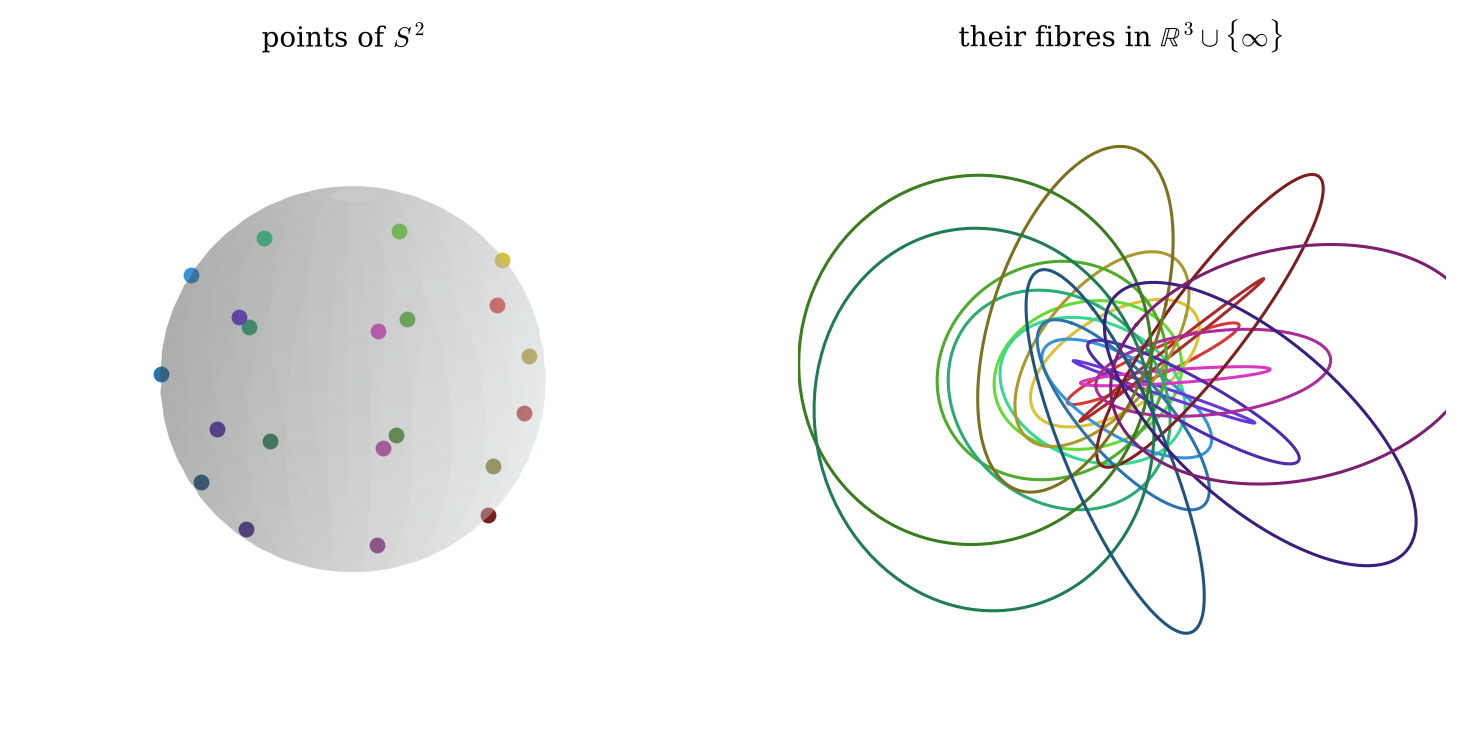
\includegraphics[width=0.92\textwidth]{fig_base_and_fibres.png}
\caption{Left: points on the base $S^2$. Right: the corresponding fibres of $h\colon S^3\to S^2$ after stereographic projection to $\R^3$, in the same colours. Points on one circle of latitude give fibres on one torus; the north pole gives the circle at infinity (here the vertical axis together with $\infty$), and the south pole gives the unit circle in the horizontal plane.}
\label{fig:basefibres}
\end{figure}

\subsection{The projective plane of the bundle}\label{sec:projplane}

For $d\ge2$ let $D(L_\K)$ be the unit disc bundle. It is a compact $2d$-manifold with boundary $S(L_\K)=S^{2d-1}$, and we put
\begin{equation}\label{eq:KP2}
\KP^2=D(L_\K)\cup_{S^{2d-1}}D^{2d},
\end{equation}
glued along the identity of $S^{2d-1}=\partial D^{2d}$. For $\K=\C,\Hq$ this is the complex or quaternionic projective plane, and for $\K=\Oc$ it is the Cayley plane;\footnote{We only use the topological description \eqref{eq:KP2}, which makes no reference to octonionic lines in $\Oc^3$.} we keep the notation $\KP^2$ in all three cases.

\begin{proposition}\label{prop:cone}
Let $d\in\{2,4,8\}$.
\begin{enumerate}[label=\textup{(\roman*)}]
\item $\KP^2$ is a closed, simply connected, hence orientable, topological $2d$-manifold.
\item $\KP^2$ is homeomorphic to the mapping cone $C_{h}=S^d\cup_{h_\K}D^{2d}$ of $h_\K$.
\item $H^j(\KP^2;\Z)\cong\Z$ for $j=0,d,2d$ and $H^j(\KP^2;\Z)=0$ otherwise.
\end{enumerate}
\end{proposition}

\begin{proof}
(ii) The disc bundle $D(L_\K)$ is homeomorphic to the mapping cylinder of the projection $S(L_\K)\to S^d$: the map $(v,t)\mapsto tv$ from $S(L_\K)\times[0,1]$ onto $D(L_\K)$ identifies exactly the points with $t=0$ in the same fibre. Gluing $D^{2d}$ to the mapping cylinder along its free end $S(L_\K)=S^{2d-1}$ gives the mapping cone.
(i) A manifold with boundary glued to another along a homeomorphism of their boundaries is a manifold, since boundaries have collar neighbourhoods. The space is compact and has no boundary. By (ii) it is a CW complex with one cell in each of the dimensions $0$, $d$ and $2d$; as $d\ge2$ there are no $1$-cells, so it is simply connected, and a simply connected manifold is orientable.
(iii) The cellular cochain complex has one generator in each of the degrees $0,d,2d$ and all differentials zero, because no two cells have adjacent dimensions.
\end{proof}

\section{The Hopf invariant}\label{ch:invariant}

This section proves Theorem~\ref{thm:B}. Section~\ref{sec:hdef} defines the invariant and proves the rules for composition that are used throughout; Section~\ref{sec:powers} computes the degree of the octonionic power maps.

\subsection{Definition and composition rules}\label{sec:hdef}

Let $n\ge2$ and $f\colon S^{2n-1}\to S^n$. The mapping cone $C_f=S^n\cup_fD^{2n}$ is a CW complex with cells in dimensions $0$, $n$ and $2n$, so
\[
H^n(C_f;\Z)\cong\Z\,\alpha_f,\qquad H^{2n}(C_f;\Z)\cong\Z\,\beta_f,
\]
where $\alpha_f$ restricts to the chosen generator of $H^n(S^n)$ and $\beta_f$ corresponds to the chosen generator of $H^{2n}(D^{2n},S^{2n-1})$ under the isomorphisms $H^{2n}(C_f)\cong H^{2n}(C_f,S^n)\cong H^{2n}(D^{2n},S^{2n-1})$.

\begin{definition}\label{def:hopfinv}
The \emph{Hopf invariant} $\Hopf(f)\in\Z$ is defined by $\alpha_f\smile\alpha_f=\Hopf(f)\,\beta_f$.
\end{definition}

If $f\simeq f'$, then $C_f$ and $C_{f'}$ are homotopy equivalent by a map that is the identity on $S^n$ and of degree one on the top cell, so $\Hopf(f)$ depends only on the homotopy class of $f$. Changing the orientation of $S^{2n-1}$ changes the sign of $\Hopf$, and changing that of $S^n$ does not. The function $\Hopf\colon\pi_{2n-1}(S^n)\to\Z$ is a homomorphism \cite[Proposition~4B.1]{Hat02}; we use this only in Corollary~\ref{cor:image} and in Section~\ref{ch:stable}.

\begin{proposition}\label{prop:hodd}
If $n$ is odd then $\Hopf(f)=0$ for every $f\colon S^{2n-1}\to S^n$.
\end{proposition}

\begin{proof}
By graded commutativity $\alpha_f^2=(-1)^{n^2}\alpha_f^2=-\alpha_f^2$, so $2\Hopf(f)\beta_f=0$ in $H^{2n}(C_f)\cong\Z$.
\end{proof}

\begin{proposition}[Composition]\label{prop:composition}
Let $f\colon S^{2n-1}\to S^n$, let $g\colon S^{2n-1}\to S^{2n-1}$ have degree $m$ and let $\varphi\colon S^n\to S^n$ have degree $k$. Then
\[
\Hopf(f\circ g)=m\,\Hopf(f),\qquad \Hopf(\varphi\circ f)=k^2\,\Hopf(f).
\]
\end{proposition}

\begin{proof}
Let $\hat g\colon D^{2n}\to D^{2n}$, $\hat g(tu)=t\,g(u)$, be the cone on $g$. It maps $S^{2n-1}$ to itself by $g$, and as a map of pairs $(D^{2n},S^{2n-1})\to(D^{2n},S^{2n-1})$ it has degree $m$, by the five lemma applied to the long exact sequences of the pairs and the boundary isomorphism $H^{2n}(D^{2n},S^{2n-1})\cong H^{2n-1}(S^{2n-1})$. The identity of $S^n$ together with $\hat g$ defines a map $\Phi\colon C_{f\circ g}\to C_f$, since a point $u\in\partial D^{2n}$ is attached at $f(g(u))$ in $C_{f\circ g}$ and $\hat g(u)=g(u)$ is attached at $f(g(u))$ in $C_f$:
\[
\begin{tikzcd}
S^{2n-1}\arrow[r,"g"]\arrow[d,hook] & S^{2n-1}\arrow[d,hook]\arrow[r,"f"] & S^n\\
D^{2n}\arrow[r,"\hat g"] & D^{2n} &
\end{tikzcd}
\qquad\leadsto\qquad
\Phi\colon C_{f\circ g}=S^n\cup_{fg}D^{2n}\longrightarrow S^n\cup_fD^{2n}=C_f .
\]
Then $\Phi^*\alpha_f=\alpha_{fg}$ and $\Phi^*\beta_f=m\beta_{fg}$, so applying $\Phi^*$ to $\alpha_f^2=\Hopf(f)\beta_f$ gives $\alpha_{fg}^2=m\Hopf(f)\beta_{fg}$. For the second identity let $\Psi\colon C_f\to C_{\varphi f}$ be $\varphi$ on $S^n$ and the identity on $D^{2n}$. Then $\Psi^*\alpha_{\varphi f}=k\alpha_f$ and $\Psi^*\beta_{\varphi f}=\beta_f$, and applying $\Psi^*$ to $\alpha_{\varphi f}^2=\Hopf(\varphi f)\beta_{\varphi f}$ gives $k^2\Hopf(f)\beta_f=\Hopf(\varphi f)\beta_f$.
\end{proof}

\begin{proposition}\label{prop:whiteheadH}
If $n$ is even, then $\Hopf([\iota_n,\iota_n])=\pm2$.
\end{proposition}

\begin{proof}
Write $S^n\times S^n=(S^n\vee S^n)\cup_wD^{2n}$ as in Section~\ref{ch:foundations}, and let $q\colon S^n\times S^n\to C=C_{\nabla\circ w}$ be the fold map $\nabla$ on $S^n\vee S^n$ and the identity on the top cell; it is well defined for the same reason as $\Phi$ above. Let $a,b\in H^n(S^n\times S^n)$ be the pull-backs of the generator along the two projections. Restriction to the $n$-skeleton is an isomorphism on $H^n$ for both spaces, and $\nabla^*$ sends the generator to $a+b$; hence $q^*\alpha=a+b$, where $\alpha=\alpha_{\nabla w}$. On the top cell $q$ is the identity, so $q^*\beta=\pm ab$, since $ab$ generates $H^{2n}(S^n\times S^n)$ by the K\"unneth theorem. Now $a^2=b^2=0$, as they are pulled back from $H^{2n}(S^n)=0$, and $ba=(-1)^{n^2}ab=ab$ since $n$ is even, so
\[
q^*(\alpha^2)=(a+b)^2=ab+ba=2ab=\pm2\,q^*\beta .
\]
As $q^*$ is an isomorphism on $H^{2n}$, $\alpha^2=\pm2\beta$.
\end{proof}

\subsection{Hopf invariant one}\label{sec:hone}

\begin{proof}[Proof of Theorem~\ref{thm:B}\textup{(i)}]
By Proposition~\ref{prop:cone}(ii) the mapping cone of $h_\K$ is homeomorphic to $\KP^2$, a closed simply connected $2d$-manifold, by a homeomorphism that is the identity on $S^d$ and of degree $\pm1$ on the top cell. Its cohomology is free, and by Poincar\'e duality (input (I2), in the form \cite[Proposition~3.38]{Hat02}) the cup product pairing $H^d(\KP^2)\times H^d(\KP^2)\to H^{2d}(\KP^2)\cong\Z$ is nonsingular. Since $H^d$ is generated by $\alpha$, this says $\alpha^2=\pm\beta$.
\end{proof}

\begin{remark}
The proof uses that $C_{h}$ is a manifold, and so it applies to any fibre bundle $p\colon S^{2d-1}\to S^d$ with fibre $S^{d-1}$, $d\ge2$: coning the fibres turns $p$ into a bundle with fibre $D^d$, which is a manifold with boundary $S^{2d-1}$, and gluing $D^{2d}$ gives a closed manifold homeomorphic to $C_p$. With Adams' theorem (I4) this gives the following statement, quoted in the Introduction.
\end{remark}

\begin{corollary}\label{cor:spherebundles}
If $S^{d-1}\to S^{2d-1}\xrightarrow{\,p\,}S^d$ is a fibre bundle with $d\ge2$, then $\Hopf(p)=\pm1$ and $d\in\{2,4,8\}$.
\end{corollary}

\subsection{Power maps}\label{sec:powers}

By Artin's theorem the powers $x^m$ of an octonion are well defined, since $x$ generates an associative subalgebra. For $d\in\{2,4,8\}$ let
\[
p_m\colon S^{d-1}\to S^{d-1},\qquad p_m(x)=x^m ,
\]
which takes values in the unit sphere by \ref{D:norm}. Every $x\in S^{d-1}\setminus\{\pm1\}$ can be written uniquely as $x=\cos\theta+u\sin\theta$ with $0<\theta<\pi$ and $u$ a unit vector orthogonal to $1$; such a $u$ satisfies $u^2=-1$ by \ref{D:conj}, so $\C_u=\R\oplus\R u$ is a subalgebra isomorphic to $\C$, and $x^m=\cos m\theta+u\sin m\theta$.

\begin{lemma}\label{lem:powerderiv}
Let $x=\cos\theta+u\sin\theta$ as above and let $W_u\subset\K$ be the orthogonal complement of $\C_u$. Then $W_u$ is tangent to $S^{d-1}$ at $x$ and at $x^m$, and
\[
Dp_m(x)(w)=\frac{\sin m\theta}{\sin\theta}\,w\qquad(w\in W_u),\qquad Dp_m(x)(ux)=m\,u\,x^m .
\]
\end{lemma}

\begin{proof}
The second formula is the derivative of $e^{i\theta}\mapsto e^{im\theta}$ in $\C_u$, since $ux=\frac{d}{d\theta}x$. For the first, $x$ and $w$ lie in a subalgebra that is associative by Artin's theorem, so $Dp_m(x)(w)=\sum_{j=0}^{m-1}x^jwx^{m-1-j}$, computed by expanding $(x+tw)^m$. Since $w\perp1$ and $w\perp u$, \ref{D:inner} gives $\Re(w)=0$ and $\Re(u\bar w)=0$, hence $\bar w=-w$ and $uw=-wu$ (the latter because $uw+wu=-(u\bar w+w\bar u)=-2\langle u,w\rangle=0$). Therefore $wx=\bar xw$, and $x^jwx^{m-1-j}=x^j\bar x^{m-1-j}w=x^{2j-m+1}w$ because $\bar x=x^{-1}$ in $\C_u$. Finally
\[
\sum_{j=0}^{m-1}x^{2j-m+1}=\sum_{j=0}^{m-1}\bigl(\cos(2j-m+1)\theta+u\sin(2j-m+1)\theta\bigr)=\frac{\sin m\theta}{\sin\theta},
\]
the sine terms cancelling in pairs $j\leftrightarrow m-1-j$. The vectors $w\in W_u$ are orthogonal to $x$ and to $x^m$, both of which lie in $\C_u$, so they are tangent to the sphere at both points.
\end{proof}

\begin{proposition}\label{prop:powerdegree}
For $d\in\{2,4,8\}$ and $m\ge1$ the power map $p_m$ has degree $m$.
\end{proposition}

\begin{proof}
Let $y=\cos\varphi+v\sin\varphi$ with $0<\varphi<\pi$, a non-real point of $S^{d-1}$. If $x^m=y$, then $y\in\C_x$, and $\C_x=\C_y=\R\oplus\R y$ because a two-dimensional subalgebra containing the non-real element $y$ is spanned by $1$ and $y$. So the solutions of $x^m=y$ are the $m$ roots of $y$ in the circle $\C_y\cap S^{d-1}$, and none of them is real. Write such a root as $x=\cos\theta+v\sin\theta$ with $\theta\in(-\pi,\pi)\setminus\{0\}$; the formulas of Lemma~\ref{lem:powerderiv} are unchanged under $(u,\theta)\mapsto(-u,-\theta)$, so they hold with $u=v$. We have $\sin\theta\ne0$ and $\sin m\theta=\pm\sin\varphi\ne0$. By Lemma~\ref{lem:powerderiv}, in the bases $(vx,w_1,\dots,w_{d-2})$ of $T_xS^{d-1}$ and $(vy,w_1,\dots,w_{d-2})$ of $T_yS^{d-1}$, with $(w_j)$ a fixed basis of $W_v$, the derivative is $\operatorname{diag}(m,c,\dots,c)$ with $c=\sin m\theta/\sin\theta\ne0$. Its determinant $m\,c^{d-2}$ is positive, since $d-2\in\{0,2,6\}$ is even. Both bases are positively oriented or both negatively: the frames $(x,vx,w_1,\dots)$ and $(y,vy,w_1,\dots)$ of $\R^d$ differ by a rotation of the plane $\C_v$ that fixes $W_v$. So $y$ is a regular value with $m$ preimages, each counted with sign $+1$.
\end{proof}

\begin{remark}
The scalar $c=\sin m\theta/\sin\theta$ vanishes at $\theta=k\pi/m$, $0<k<m$, where $x^m=\pm1$; the critical points of $p_m$ for $d\ge4$ form the $(d-2)$-spheres $\{\cos(k\pi/m)+u\sin(k\pi/m):u\perp1,\ |u|=1\}$, which $p_m$ collapses to the points $(-1)^k$. For $d=2$ there are no critical points.
\end{remark}

\begin{proposition}\label{prop:gm}
For $d\in\{2,4,8\}$ and $m\ge1$ the map $g_m\colon S^{2d-1}\to S^{2d-1}$, $g_m(a,b)=(a^m,b)/|(a^m,b)|$, has degree $m$, and it fixes the point $(1,0)$. The map $\kappa(a,b)=(\bar a,b)$ has degree $-1$.
\end{proposition}

\begin{proof}
Write $a=\rho x$ with $\rho=|a|$ and $|x|=1$. For $t\in[0,1]$ the maps
\[
F_t(\rho x,b)=\bigl(\rho^{(1-t)m+t}x^m,\;b\bigr)
\]
are continuous on $\K^2$ (the exponent is at least $1$) and vanish only at $0$, so $F_t/|F_t|$ is a homotopy of self-maps of $S^{2d-1}$ fixing $(1,0)$, from $g_m$ to $g'(a,b)=(|a|\,p_m(a/|a|),\,b)$, extended by $g'(0,b)=(0,b)$; note that $(|a|\,p_m(a/|a|),b)$ already has norm one. On the open dense subset $\{a\neq0,\ b\neq0\}$ of $S^{2d-1}$ we use the diffeomorphism
\[
(0,\tfrac{\pi}{2})\times S^{d-1}\times S^{d-1}\to\{a\ne0,b\ne0\},\qquad (s,x,z)\mapsto(x\cos s,\;z\sin s),
\]
in which $g'$ becomes $(s,x,z)\mapsto(s,p_m(x),z)$. A regular value $y$ of $p_m$ gives a regular value $(y\cos s,z\sin s)$ of $g'$, whose preimages $(x\cos s,z\sin s)$, $x^m=y$, are $m$ points at which the Jacobian in these coordinates has the sign of $\det Dp_m(x)$, that is $+1$. The same chart is used in source and target, so the sign relative to the orientation of $S^{2d-1}$ is also $+1$, and $\deg g_m=\deg g'=m$. The map $\kappa$ is the restriction of a linear map of $\R^{2d}$ that negates the $d-1$ imaginary coordinates of $a$, so its degree is $(-1)^{d-1}=-1$.
\end{proof}

\begin{proof}[Proof of Theorem~\ref{thm:B}\textup{(ii)} and \textup{(iii)}]
Part (ii) is Propositions~\ref{prop:powerdegree} and \ref{prop:gm}. Since $g_m$ is a based map of degree $m$, Lemma~\ref{lem:precompose} gives $[h_\K\circ g_m]=m[h_\K]$ in $\pi_{2d-1}(S^d)$, and Proposition~\ref{prop:composition} gives $\Hopf(h_\K\circ g_m)=m\Hopf(h_\K)=\pm m$ and $\Hopf(h_\K\circ g_m\circ\kappa)=\mp m$. Because $h_\K(\lambda v)=\lambda^2h_\K(v)$ for real $\lambda$,
\begin{equation}\label{eq:hgm}
h_\K\circ g_m(a,b)=\frac{\bigl(2a^m\bar b,\;|a|^{2m}-|b|^2\bigr)}{|a|^{2m}+|b|^2},
\end{equation}
whose numerator and denominator are polynomials in the real coordinates of $(a,b)$. With the constant map for $0$, every integer is the Hopf invariant of such a map.
\end{proof}

\begin{corollary}\label{cor:image}
The image of $\Hopf\colon\pi_{2n-1}(S^n)\to\Z$ is $0$ for $n$ odd, $\Z$ for $n=2,4,8$, and $2\Z$ for every other even $n$.
\end{corollary}

\begin{proof}
The first case is Proposition~\ref{prop:hodd}. For $n$ even the image is a subgroup containing $2$ by Proposition~\ref{prop:whiteheadH}, so it is $\Z$ or $2\Z$; it is $\Z$ for $n=2,4,8$ by Theorem~\ref{thm:B}(i), and $2\Z$ otherwise by Adams' theorem (I4).
\end{proof}

\begin{remark}\label{rem:whitehead-hopf}
For $n=2$ the group $\pi_3(S^2)\cong\Z$ (Theorem~\ref{thm:C}) is detected by $\Hopf$, so Proposition~\ref{prop:whiteheadH} gives $[\iota_2,\iota_2]=\pm2[h]$. For $n=4$ it gives $[\iota_4,\iota_4]\equiv\pm2[h_\Hq]$ modulo the torsion subgroup $\Z/12$ of $\pi_7(S^4)$; the exact formula $[\iota_4,\iota_4]=2\nu_4-E\nu'$ in Toda's notation is \cite[Chapter~V]{Tod62}. Proposition~\ref{prop:composition} also shows that $\Hopf(h\circ\varphi)=k$ for a self-map $\varphi$ of $S^3$ of degree $k$, while $\Hopf(\varphi'\circ h)=k^2$ for a self-map $\varphi'$ of $S^2$ of degree $k$; both appear again in Section~\ref{ch:linking}, as $[z^k:w]$ and $[z^k:w^k]$.
\end{remark}

\section{Homotopy groups from the Hopf bundles}\label{ch:groups}

\subsection{The splitting}

\begin{proof}[Proof of Theorem~\ref{thm:C}]
Let $d\in\{2,4,8\}$ and let $F=h_\K^{-1}(N_0)=\{(a,0):|a|=1\}\cong S^{d-1}$ be the fibre over the north pole. By Corollary~\ref{cor:fibration}, $h_\K$ is a fibration. The inclusion $j\colon F\to S^{2d-1}$ is null-homotopic, because $\pi_{d-1}(S^{2d-1})=0$ by Proposition~\ref{prop:below}; explicitly,
\begin{equation}\label{eq:nullhomotopy}
G\colon F\times[0,\tfrac\pi2]\to S^{2d-1},\qquad G(a,s)=(a\cos s,\;\sin s)
\end{equation}
contracts $F$ to the point $(0,1)$. All three spaces are path connected, and $\pi_{i-1}(S^{d-1})$ is abelian for $i\ge2$ (it is $\pi_1(S^1)\cong\Z$ or zero when $i=2$). Lemma~\ref{lem:split} gives the split exact sequence
\[
0\to\pi_i(S^{2d-1})\xrightarrow{(h_\K)_*}\pi_i(S^d)\xrightarrow{\ \partial\ }\pi_{i-1}(S^{d-1})\to0 .
\]
For $d=2$ and $i\ge3$ the third group is $\pi_{i-1}(S^1)=0$ by Example~\ref{ex:covering}, so $(h_\C)_*$ is an isomorphism. The values $\pi_6(S^3)\cong\Z/12$, $\pi_7(S^3)\cong\Z/2$ and $\pi_{14}(S^7)\cong\Z/120$ are taken from Toda's tables (I6), \cite[Chapter~XIV]{Tod62}, and give $\pi_7(S^4)\cong\Z\oplus\Z/12$, $\pi_8(S^4)\cong(\Z/2)^2$ and $\pi_{15}(S^8)\cong\Z\oplus\Z/120$. The infinite cyclic summand of $\pi_{2d-1}(S^d)$ is $(h_\K)_*\pi_{2d-1}(S^{2d-1})$, generated by $[h_\K]$, and by Proposition~\ref{prop:composition} the Hopf invariant of $(h_\K)_*[g]=[h_\K\circ g]$ is $\pm\deg g$; so it detects this summand.
\end{proof}

The splitting map of Lemma~\ref{lem:split} can be identified.

\begin{proposition}\label{prop:sigmaE}
For the null-homotopy \eqref{eq:nullhomotopy}, the splitting $\sigma\colon\pi_{i-1}(S^{d-1})\to\pi_i(S^d)$ of \eqref{eq:sigma} is the suspension homomorphism $E$, up to a sign that depends only on orientation conventions. Hence
\[
\pi_i(S^d)=(h_\K)_*\pi_i(S^{2d-1})\;\oplus\;E\,\pi_{i-1}(S^{d-1})\qquad(d=2,4,8,\ i\ge2),
\]
and the suspensions $E\colon\pi_{i-1}(S^3)\to\pi_i(S^4)$ and $E\colon\pi_{i-1}(S^7)\to\pi_i(S^8)$ are injective for every $i$.
\end{proposition}

\begin{proof}
Composing $G$ with $h_\K$ gives
\[
h_\K\bigl(G(a,s)\bigr)=\bigl(2a\cos s\sin s,\;\cos^2s-\sin^2s\bigr)=\bigl(a\sin2s,\;\cos2s\bigr),
\]
which, as $s$ runs from $0$ to $\pi/2$, moves the point $a$ of the fibre along the meridian of $S^d$ from the north pole through the direction $a$ to the south pole. For $\beta\colon S^{i-2}\to F$, the element $\sigma[\beta]$ is represented by $(u,s)\mapsto(\beta(u)\sin2s,\cos2s)$ on $S^{i-2}\times[0,\pi/2]$, which collapses $S^{i-2}\times\{0\}$ to the north pole and $S^{i-2}\times\{\pi/2\}$ to the south pole. This is the unreduced suspension of $\beta$ followed by the identification $\Sigma S^{d-1}\cong S^d$ given by meridians; as an element of $\pi_i(S^d)$ it is $\pm E[\beta]$, the unreduced and reduced suspensions being homotopy equivalent. The last statement holds because $\sigma=\pm E$ is a split injection.
\end{proof}

\begin{remark}
For $d=2$ and $i=2$ the proposition gives $\pi_2(S^2)=E\pi_1(S^1)\cong\Z$, generated by $E[\mathrm{id}_{S^1}]=[\mathrm{id}_{S^2}]$, in accordance with Proposition~\ref{prop:degree}. For $d=4$ it recovers the classical decomposition $\pi_i(S^4)\cong\pi_i(S^7)\oplus\pi_{i-1}(S^3)$ with the second summand embedded by suspension \cite[Chapter~V]{Tod62}.
\end{remark}

\subsection{The table of unstable groups}\label{sec:table}

Table~\ref{tab:unstable} lists $\pi_{n+k}(S^n)$ for $k\le7$ and $n\le9$, with the stable value in the last column. All entries are taken from Toda \cite{Tod62}, but the entries in the columns $n=2,4,8$ are also consequences of Theorem~\ref{thm:C} and the entries in the columns $n=3$, $n=7$; the columns $n\ge k+2$ are constant by Freudenthal's theorem. Figure~\ref{fig:table} shows the same table with the three kinds of entries distinguished. That the table is consistent with Theorem~\ref{thm:C} and with Theorem~\ref{thm:freudenthal}, as abelian groups, is checked by the program of Appendix~\ref{app:checks}.

\begin{table}[ht]
\centering
\small
\setlength{\tabcolsep}{4.2pt}
\begin{tabular}{@{}c|ccccccccc|c@{}}
\toprule
$k\backslash n$ & $1$ & $2$ & $3$ & $4$ & $5$ & $6$ & $7$ & $8$ & $9$ & $\pi_k^s$\\
\midrule
$0$ & $\Z$ & $\Z$ & $\Z$ & $\Z$ & $\Z$ & $\Z$ & $\Z$ & $\Z$ & $\Z$ & $\Z$\\
$1$ & $0$ & $\Z$ & $2$ & $2$ & $2$ & $2$ & $2$ & $2$ & $2$ & $2$\\
$2$ & $0$ & $2$ & $2$ & $2$ & $2$ & $2$ & $2$ & $2$ & $2$ & $2$\\
$3$ & $0$ & $2$ & $12$ & $\Z{\oplus}12$ & $24$ & $24$ & $24$ & $24$ & $24$ & $24$\\
$4$ & $0$ & $12$ & $2$ & $2^2$ & $2$ & $0$ & $0$ & $0$ & $0$ & $0$\\
$5$ & $0$ & $2$ & $2$ & $2^2$ & $2$ & $\Z$ & $0$ & $0$ & $0$ & $0$\\
$6$ & $0$ & $2$ & $3$ & $24{\oplus}3$ & $2$ & $2$ & $2$ & $2$ & $2$ & $2$\\
$7$ & $0$ & $3$ & $15$ & $15$ & $30$ & $60$ & $120$ & $\Z{\oplus}120$ & $240$ & $240$\\
\bottomrule
\end{tabular}
\caption{The groups $\pi_{n+k}(S^n)$ for $0\le k\le7$, after Toda \cite{Tod62}; an integer $m$ stands for $\Z/m$ and $2^2$ for $(\Z/2)^2$. The column $n=2$ equals the column $n=3$ shifted down by one row; the column $n=4$ is the sum of the column $n=7$ shifted down by three rows and the column $n=3$; the column $n=8$ is the sum of the column $n=7$ and the group $\pi_{8+k}(S^{15})$, which is $\Z$ for $k=7$ and $0$ for $k<7$.}
\label{tab:unstable}
\end{table}

\begin{figure}[ht]
\centering
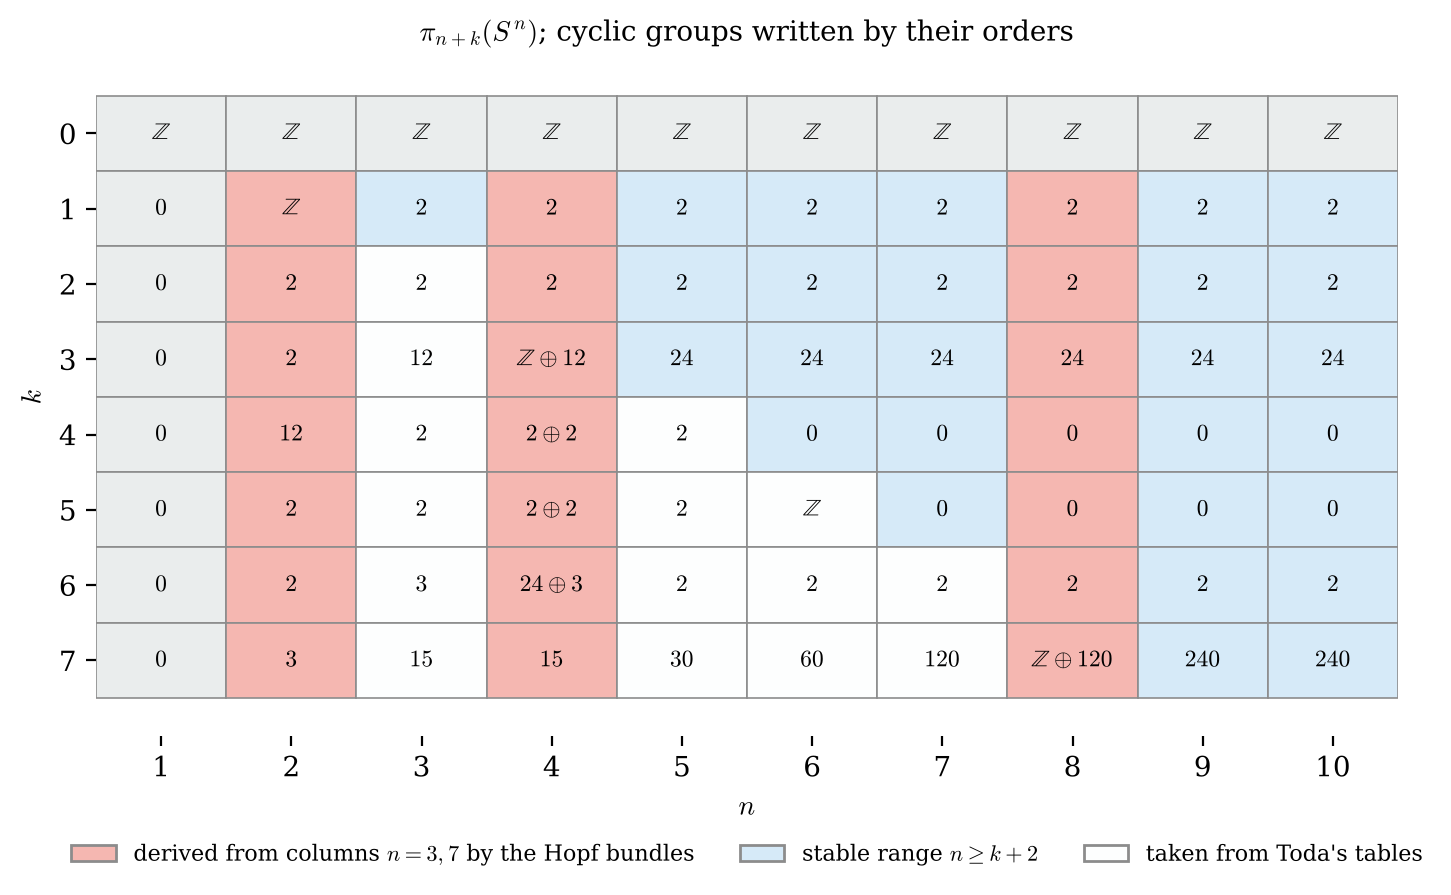
\includegraphics[width=0.95\textwidth]{fig_table.png}
\caption{The table of $\pi_{n+k}(S^n)$. Dark cells are derived from the columns $n=3$ and $n=7$ by the Hopf bundles (Theorem~\ref{thm:C}); light cells lie in the stable range $n\ge k+2$ (Theorem~\ref{thm:freudenthal}); white cells are taken from Toda's tables.}
\label{fig:table}
\end{figure}

\begin{example}\label{ex:derived}
Reading the table through Theorem~\ref{thm:C}:
\begin{enumerate}[label=\textup{(\alph*)}]
\item $\pi_4(S^2)\cong\pi_4(S^3)\cong\Z/2$, $\pi_5(S^2)\cong\pi_5(S^3)\cong\Z/2$, $\pi_6(S^2)\cong\pi_6(S^3)\cong\Z/12$.
\item $\pi_8(S^4)\cong\pi_8(S^7)\oplus\pi_7(S^3)\cong(\Z/2)^2$ and $\pi_9(S^4)\cong\pi_9(S^7)\oplus\pi_8(S^3)\cong(\Z/2)^2$.
\item $\pi_{10}(S^4)\cong\pi_{10}(S^7)\oplus\pi_9(S^3)\cong\Z/24\oplus\Z/3$.
\item $\pi_{i}(S^8)\cong\pi_{i-1}(S^7)$ for $8\le i\le14$, and $\pi_{15}(S^8)\cong\Z\oplus\Z/120$.
\end{enumerate}
In each case the summand $\pi_i(S^{2d-1})$ is the image of composition with the Hopf map, and the summand $\pi_{i-1}(S^{d-1})$ is the image of the suspension.
\end{example}

\subsection{Generators}\label{sec:generators}

In Toda's notation \cite{Tod62} the Hopf maps are $\eta_2=[h_\C]$, $\nu_4=[h_\Hq]$ and $\sigma_8=[h_\Oc]$, and $\eta_n$, $\nu_n$, $\sigma_n$ denote their iterated suspensions. The stable stems in degrees $1$, $3$ and $7$ are cyclic of orders $2$, $24$ and $240$, generated by $\eta$, $\nu$ and $\sigma$ \cite[Chapters~V and XIV]{Tod62}. Before suspension the Hopf maps have infinite order, since their Hopf invariant is $\pm1$ (Theorem~\ref{thm:B}); after suspension they have finite order and generate the image of the $J$-homomorphism in these degrees (Section~\ref{ch:stable}). For instance, $E^2\nu'=2\nu_5$ for the generator $\nu'$ of $\pi_6(S^3)\cong\Z/12$ \cite[Chapter~V]{Tod62}, so the summand $E\pi_6(S^3)$ of $\pi_7(S^4)$ maps onto the subgroup of index two of $\pi_8(S^5)\cong\Z/24$, and the summand $\Z\nu_4$ maps onto the whole group.

\chapter{Linking and holomorphic maps}\label{ch:linking}

\section{Linking numbers}\label{sec:lk}

Let $K_1,K_2\subset S^3$ be disjoint oriented closed $1$-manifolds. Since $H_1(S^3)=0$, $K_1$ bounds an oriented surface $\Sigma$ (a Seifert surface, or more generally a $2$-chain), which may be chosen transverse to $K_2$, and the \emph{linking number} $\lk(K_1,K_2)$ is the algebraic intersection number $\Sigma\cdot K_2$. It does not depend on $\Sigma$, it is symmetric, and for $K_1,K_2\subset\R^3$ it is given by the Gauss integral
\begin{equation}\label{eq:gauss}
\lk(K_1,K_2)=\frac1{4\pi}\oint_{K_1}\oint_{K_2}\frac{(\mathbf x-\mathbf y)\cdot(d\mathbf x\times d\mathbf y)}{|\mathbf x-\mathbf y|^3}.
\end{equation}
The integral \eqref{eq:gauss} is used in Appendix~\ref{app:checks} to check the computations of this chapter numerically.

Orient the fibres of $h\colon S^3\to S^2$ by the circle action $\lambda\mapsto(\lambda z,\lambda w)$.

\begin{proposition}\label{prop:fibrelink}
Any two distinct fibres of $h$ have linking number $\varepsilon$, where $\varepsilon\in\{\pm1\}$ depends only on the orientation of $S^3$.
\end{proposition}

\begin{proof}
The fibre over the north pole $N_0$ is $C_\infty=\{(z,0):|z|=1\}$. It bounds the hemisphere
\[
\Sigma=\{(z,t)\in S^3:t\in\R,\ t\ge0\},
\]
a $2$-disc. By Corollary~\ref{cor:fibration} the fibre over $s(x)$, $x\in\C$, is $C_x=\{(xc,c):|c|=(1+|x|^2)^{-1/2}\}$, and it meets $\Sigma$ exactly where $c$ is real and positive, at one point. The intersection is transverse: along $C_x$, written as $c=\rho e^{i\phi}$, the function $\Imag w=\rho\sin\phi$ that cuts out $\Sigma$ near the intersection has nonzero derivative $\rho$ at $\phi=0$. So $\lk(C_\infty,C_x)=\pm1$, and the sign is constant in $x$ because $\C$ is connected and the fibres $C_x$ vary continuously. Now let $C_p,C_q$ be any two distinct fibres. The group $\U(2)$ acts on $S^3$ by orientation-preserving isometries commuting with the circle action, so it permutes the oriented fibres, and it acts transitively on $S^2$ through $\U(2)\to\SO(3)$. Choosing $g\in\U(2)$ with $gC_p=C_\infty$ gives $\lk(C_p,C_q)=\lk(C_\infty,gC_q)$, which is the constant found above.
\end{proof}

The connection with the Hopf invariant is Hopf's original definition \cite{Hop31}; see \cite[Section~17]{BT82} for a proof.

\begin{theorem}[Linking formula]\label{thm:linkingformula}
Let $f\colon S^3\to S^2$ be smooth and let $p\neq q$ be regular values. Orient $f^{-1}(p)$ and $f^{-1}(q)$ as preimages. Then $\Hopf(f)=\pm\lk(f^{-1}(p),f^{-1}(q))$, with a universal sign.
\end{theorem}

We fix the orientation of $S^3$ (the boundary orientation of the unit ball in $\C^2$ with its complex orientation) and choose the generators in Definition~\ref{def:hopfinv} so that $\Hopf(h)=1$. With these choices the universal sign is $\varepsilon$, by Proposition~\ref{prop:fibrelink} applied to $f=h$: the fibres of $h$, oriented by the circle action, are its preimages with their preimage orientation up to one fixed sign.

\begin{figure}[t]
\centering
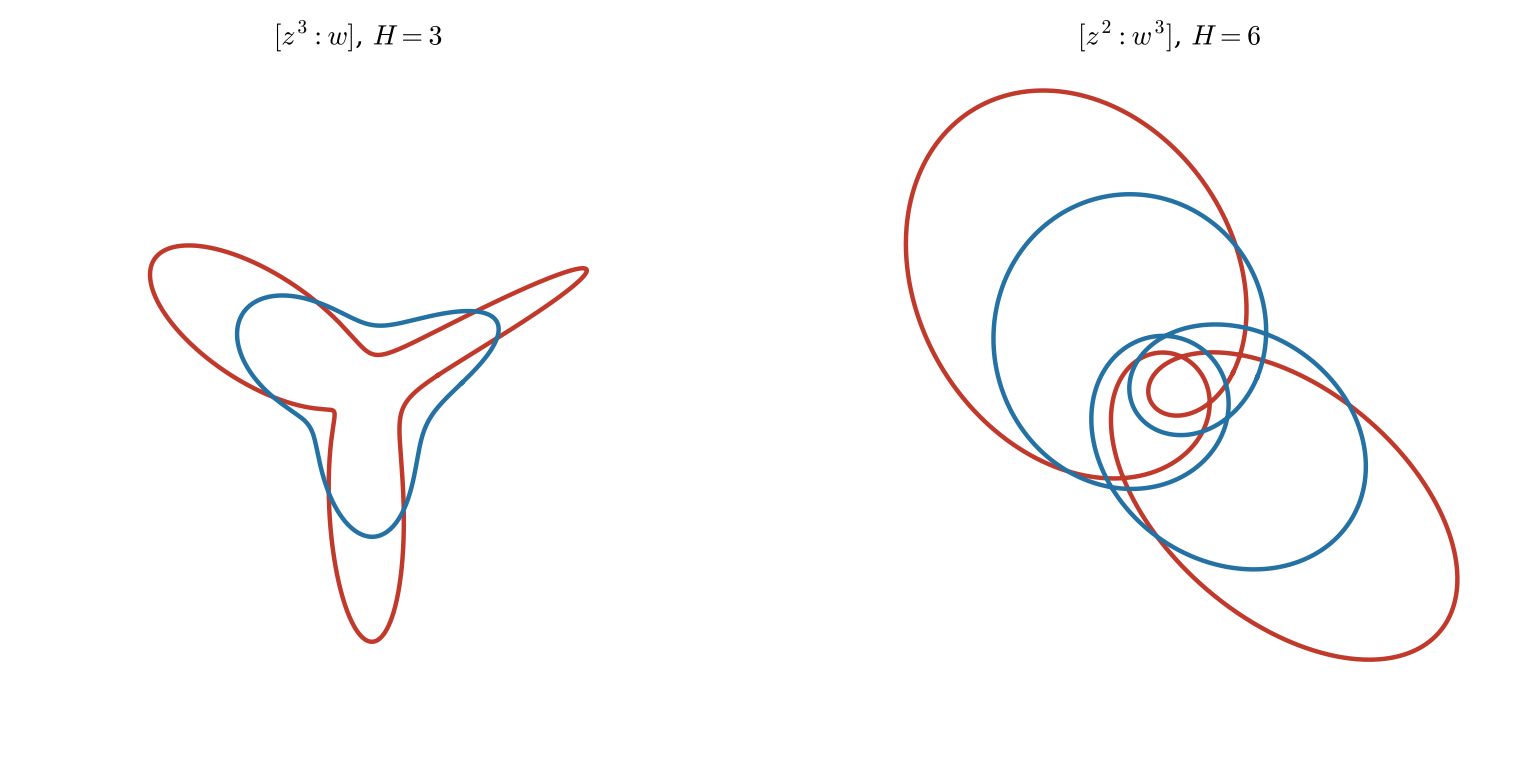
\includegraphics[width=0.95\textwidth]{fig_torus_links.png}
\caption{Two fibres of $[z^3:w]$, with Hopf invariant $3$ (left), and of $[z^2:w^3]$, with Hopf invariant $6$ (right), after stereographic projection. Each fibre lies on a torus about the axis and is a torus link of type $(p,q)$; the Gauss integral \eqref{eq:gauss} gives linking numbers $3$ and $6$ (Appendix~\ref{app:checks}).}
\label{fig:toruslinks}
\end{figure}

\section{Holomorphic maps}\label{sec:holomorphic}

Let $P,Q\in\C[z,w]$ have no common zero on $S^3$, put $F=(P,Q)\colon\C^2\to\C^2$ and
\[
[P:Q]=h\circ\frac{F}{|F|}\colon S^3\to S^2 ,
\]
which is the map $u\mapsto[P(u):Q(u)]\in\CP^1=S^2$ in the chart \eqref{eq:stereo} with $x=P/Q$; the formula of the Introduction follows from $h(\lambda v)=\lambda^2h(v)$ for real $\lambda$. Let $Z=\{u\in\C^2:P(u)=Q(u)=0\}$.

\begin{lemma}\label{lem:bounded}
Let $C\subset\C^2$ be an irreducible affine plane curve that does not meet $S^3$. Then $C$ does not meet the closed ball $\bar B^4$.
\end{lemma}

\begin{proof}
The closure of $C$ in $\CP^2$ is an irreducible projective curve, and $C$ is its complement of the finitely many points at infinity, so $C$ is connected in the classical topology \cite[Corollary~(4.16)]{Mum76}. As $C\cap S^3=\emptyset$, $C$ is the disjoint union of the open sets $C\cap B^4$ and $C\setminus\bar B^4$, so if $C$ meets $\bar B^4$ then $C\subset B^4$ is bounded. But no affine curve $C=\{D=0\}$, $D$ irreducible, is bounded. If $D$ has degree $k\ge1$ in $w$, with leading coefficient $a(z)$, then for every $z_1$ with $a(z_1)\neq0$ the polynomial $D(z_1,\cdot)$ has a root, so the projection of $C$ to the $z$-coordinate contains the complement of a finite set. If $D$ has degree $0$ in $w$, it is an irreducible polynomial in $z$ alone, that is $D=z-z_0$ up to a scalar, and $C=\{z_0\}\times\C$.
\end{proof}

\begin{lemma}[Finiteness]\label{lem:finite}
Let $D=\gcd(P,Q)$ and $P=DP'$, $Q=DQ'$. Then $Z\cap\bar B^4=\{P'=Q'=0\}\cap B^4$; this set is finite, and $I_u(P,Q)=I_u(P',Q')$ at each of its points.
\end{lemma}

\begin{proof}
$Z=\{D=0\}\cup\{P'=Q'=0\}$. Every irreducible component of $\{D=0\}$ lies in $Z$, so it does not meet $S^3$, and by Lemma~\ref{lem:bounded} it does not meet $\bar B^4$. The coprime polynomials $P',Q'$ have at most $\deg P'\cdot\deg Q'$ common zeros in $\C^2$ \cite[Section~5.3]{Ful69}, and none on $S^3$. At a point $u$ with $D(u)\neq0$, $D$ is a unit in the local ring $\mathcal O_u$, so $(P,Q)=(P',Q')$ in $\mathcal O_u$.
\end{proof}

\begin{lemma}[Degree as a sum of indices]\label{lem:indexsum}
Let $\Phi\colon\bar B^{n}\to\R^{n}$ be smooth with finitely many zeros, all in the open ball. Then the degree of $\Phi/|\Phi|\colon S^{n-1}\to S^{n-1}$ is the sum of the local indices of $\Phi$ at its zeros, where the index at $u$ is the degree of $\Phi/|\Phi|$ on a small sphere about $u$.
\end{lemma}

\begin{proof}
Remove disjoint small open balls $B_u$ about the zeros. On the compact oriented manifold $X=\bar B^n\setminus\bigcup B_u$ the map $\Phi/|\Phi|$ is defined, and its restriction to $\partial X=S^{n-1}\sqcup\bigsqcup(-\partial B_u)$ has degree zero, because it extends over $X$ \cite[Section~5, Lemma~1]{Mil65}. This is the statement, input (I5).
\end{proof}

\begin{proof}[Proof of Theorem~\ref{thm:D}]
Finiteness is Lemma~\ref{lem:finite}. The map $g=F/|F|\colon S^3\to S^3$ satisfies $[P:Q]=h\circ g$, so by Proposition~\ref{prop:composition}, $\Hopf([P:Q])=\deg(g)\Hopf(h)=\deg g$. By Lemma~\ref{lem:indexsum}, applied to $\Phi=F|_{\bar B^4}$, $\deg g$ is the sum of the indices of $F$ at the points of $Z\cap B^4$. At each such point the index of the holomorphic germ $F$ is the intersection multiplicity $I_u(P,Q)$, input (I5) \cite[Chapter~5]{GH78}, \cite[Chapter~5]{AGV85}.\footnote{When $u$ is a regular zero this is the observation that the real Jacobian of a holomorphic map is $|\det_\C DF|^2>0$, so the index is $+1$; in general one perturbs $F$ to $F-\epsilon$ for a small regular value $\epsilon$, whose $I_u(P,Q)$ preimages near $u$ are all regular.} This proves the formula. The sum is $\ge0$, and by Lemma~\ref{lem:finite} and the affine B\'ezout inequality \cite[Section~5.3]{Ful69},
\[
\sum_{u\in Z\cap B^4}I_u(P,Q)=\sum_{u\in B^4}I_u(P',Q')\le\sum_{u\in\C^2}I_u(P',Q')\le\deg P'\cdot\deg Q'\le\deg P\cdot\deg Q .
\]
For $[z^p:w^q]$ the only common zero is $0$, with $I_0(z^p,w^q)=\dim_\C\C[z,w]/(z^p,w^q)=pq$; for $[1:0]$, or any $[P:Q]$ with $Q$ a nonzero constant, there are none. Since $\pi_3(S^2)\cong\Z$ is detected by $\Hopf$ (Theorem~\ref{thm:C}), $[P:Q]$ is null-homotopic exactly when $Z\cap B^4=\emptyset$, every $I_u$ being at least one. Finally $[z^m:w]$ has Hopf invariant $m$, and for the map $\kappa(z,w)=(\bar z,w)$ of degree $-1$ the composite $[z^m:w]\circ\kappa$ has Hopf invariant $-m$ by Proposition~\ref{prop:composition}.
\end{proof}

The two inequalities in the proof give an exact criterion for the upper bound.

\begin{proposition}[Equality]\label{prop:equality}
Let $p=\deg P$ and $q=\deg Q$, and let $\tilde P,\tilde Q$ be the homogenisations in $\CP^2$. Then $\Hopf([P:Q])=pq$ if and only if $P$ and $Q$ have no common factor, $\tilde P$ and $\tilde Q$ have no common zero on the line at infinity, and all common zeros of $P$ and $Q$ in $\C^2$ lie in $B^4$.
\end{proposition}

\begin{proof}
By B\'ezout's theorem in $\CP^2$ \cite[Section~5.3]{Ful69}, two curves of degrees $p$ and $q$ without common component meet in exactly $pq$ points counted with multiplicity. If $D=\gcd(P,Q)$ is not constant, the chain of inequalities above is strict at the last step. Otherwise the sum over $\C^2$ equals $pq$ minus the multiplicities at infinity, and the sum over $B^4$ equals the sum over $\C^2$ exactly when no common zero lies outside $\bar B^4$; none lies on $S^3$ by hypothesis.
\end{proof}

\begin{example}\label{ex:holoexamples}
\begin{enumerate}[label=\textup{(\alph*)}]
\item $[z^p:w^q]$: $\Hopf=pq$. The fibre over a point $[\alpha:\beta]$ with $\alpha\beta\neq0$ lies on the torus $|z|=r_1$, $|w|=r_2$ determined by $r_1^2+r_2^2=1$ and $r_1^p|\beta|=r_2^q|\alpha|$, and there it is the set $\{p\arg z-q\arg w\equiv\arg(\alpha/\beta)\}$, the torus link of type $(p,q)$ with $\gcd(p,q)$ components. Two such fibres have linking number $pq$, as Theorem~\ref{thm:linkingformula} requires; Figure~\ref{fig:toruslinks} shows the cases $(3,1)$ and $(2,3)$.
\item If $P$ and $Q$ are homogeneous of the same degree $k$ with no common factor, the only common zero is $0$, and $I_0(P,Q)=k^2$ because the tangent cones $P$ and $Q$ have no common line \cite[Section~3.3]{Ful69}. So $\Hopf=k^2$, in accordance with $[P:Q]=\varphi\circ h$ for the rational map $\varphi=[P:Q]$ of $\CP^1$ of degree $k$ and Proposition~\ref{prop:composition}.
\item $[z^2-\tfrac14:w]$ has the common zeros $(\pm\tfrac12,0)\in B^4$, each of multiplicity one, so $\Hopf=2=\deg P\cdot\deg Q$. Moving the zeros outward, $[z^2-c^2:w]$ has $\Hopf=2$ for $|c|<1$ and $\Hopf=0$ for $|c|>1$; at $|c|=1$ the hypothesis fails, and the map is not defined everywhere.
\item $[z^2:zw+1]$: the common zeros satisfy $z=0$ and $1=0$, so there are none, and $\Hopf=0<2\cdot2$, although $P$ and $Q$ are coprime; here $\tilde P=z^2$ and $\tilde Q=zw+t^2$ meet only at $[0:1:0]$ on the line at infinity, with multiplicity four.
\end{enumerate}
\end{example}

\begin{corollary}[Linking as intersection]\label{cor:lkint}
Let $[P:Q]$ be as in Theorem~\ref{thm:D}, and let $[\alpha:\beta]\neq[\gamma:\delta]$ be regular values. Then the links $K_1=\{\beta P=\alpha Q\}\cap S^3$ and $K_2=\{\delta P=\gamma Q\}\cap S^3$ bound the holomorphic curves $C_1=\{\beta P=\alpha Q\}\cap\bar B^4$ and $C_2=\{\delta P=\gamma Q\}\cap\bar B^4$ in the ball, and
\[
\varepsilon\,\lk(K_1,K_2)=\sum_{u\in C_1\cap C_2}I_u(\beta P-\alpha Q,\ \delta P-\gamma Q)=\Hopf([P:Q]).
\]
\end{corollary}

\begin{proof}
The fibres of $[P:Q]$ over the two values are $K_1$ and $K_2$, so the first and last terms agree by Theorem~\ref{thm:linkingformula}. Since $\alpha\delta-\beta\gamma\neq0$, the ideal $(\beta P-\alpha Q,\delta P-\gamma Q)$ equals $(P,Q)$, so the middle term is the sum in Theorem~\ref{thm:D}.
\end{proof}

\begin{remark}
Corollary~\ref{cor:lkint} is a special case of the general fact that the linking number of the boundaries of two complex curves in the ball, meeting $S^3$ transversally, is their intersection number in the ball, which is a sum of positive local contributions. It explains why the holomorphic Hopf invariants are non-negative: complex curves meet positively.
\end{remark}

\section{Split quaternionic and octonionic maps}\label{sec:split}

For $\K=\Hq$ or $\Oc$ there is no algebraic intersection theory, but part of Theorem~\ref{thm:D} survives. A \emph{polynomial in one variable} over $\K$ is a function $P(a)=\sum_{k=0}^ma^kp_k$ with $p_k\in\K$; powers are well defined because a single element generates an associative subalgebra (Lemma~\ref{lem:artin}). It has degree $m$ if $p_m\neq0$. For such $P$ and $Q(b)=\sum_{k=0}^nb^kq_k$ put $F(a,b)=(P(a),Q(b))$, a map $\K^2\to\K^2$ whose zero set is $Z(P)\times Z(Q)$.

\begin{proposition}\label{prop:split}
Let $\K=\Hq$ or $\Oc$, and let $P$, $Q$ be polynomials of degrees $m,n\ge1$ in one variable such that $F$ has no zero on $S^{2d-1}$. Then $f=F/|F|\colon S^{2d-1}\to S^{2d-1}$ and the map $h_\K\circ f\colon S^{2d-1}\to S^d$ satisfy:
\begin{enumerate}[label=\textup{(\roman*)}]
\item if every zero of $F$ lies in the open ball $B^{2d}$, then $\deg f=mn$ and $\Hopf(h_\K\circ f)=mn\,\Hopf(h_\K)=\pm mn$;
\item if no zero of $F$ lies in the closed ball $\bar B^{2d}$, then $\deg f=0$ and $\Hopf(h_\K\circ f)=0$;
\item in all cases $\Hopf(h_\K\circ f)=\deg(f)\,\Hopf(h_\K)$, and $\deg f$ depends only on $P$, $Q$ and the set of zeros of $F$ in $B^{2d}$: it is unchanged by any deformation of $(P,Q)$ through such pairs during which no zero of $F$ crosses $S^{2d-1}$.
\end{enumerate}
\end{proposition}

\begin{proof}
By Proposition~\ref{prop:composition}, $\Hopf(h_\K\circ f)=\deg(f)\Hopf(h_\K)$, and $\Hopf(h_\K)=\pm1$ by Theorem~\ref{thm:B}. A deformation of the kind in (iii) is a homotopy of maps $S^{2d-1}\to S^{2d-1}$, which proves (iii). If $F$ has no zero in $\bar B^{2d}$, then $F/|F|$ extends to $\bar B^{2d}$, so $f$ is null-homotopic and (ii) follows.

For (i), let $R\ge1$. If $F$ has no zero with $1\le|(a,b)|\le R$, then $(r,v)\mapsto F(rv)/|F(rv)|$ for $r\in[1,R]$ is a homotopy from $f$ to the map $f_R(v)=F(Rv)/|F(Rv)|$, so $\deg f=\deg f_R$. Under the hypothesis of (i) this holds for every $R\ge1$. For $t\in[0,1]$ put $P_t(a)=a^mp_m+t\sum_{k<m}a^kp_k$ and similarly $Q_t$. By \ref{D:norm}, $|a^kp_k|=|a|^k|p_k|$, so
\[
|P_t(a)|\ge|a|^m|p_m|-\sum_{k<m}|a|^k|p_k|,
\]
which is positive for $|a|\ge R/\sqrt2$ once $R$ is large; the same holds for $Q_t$. Every point of the sphere of radius $R$ has $|a|\ge R/\sqrt2$ or $|b|\ge R/\sqrt2$, so $(P_t,Q_t)$ has no zero on it, and $\deg f_R$ equals the degree of $v\mapsto(a^mp_m,b^nq_n)/|(a^mp_m,b^nq_n)|$ on the sphere of radius $R$, which after the radial homotopy is the same on $S^{2d-1}$. Joining $p_m/|p_m|$ to $1$ and $|p_m|$ to $1$ by paths in $S^{d-1}$ and $(0,\infty)$, and likewise for $q_n$, does not create zeros on $S^{2d-1}$, since $a^mc=0$ forces $a=0$ for $c\neq0$. So $\deg f=\deg e_{m,n}$ with $e_{m,n}(a,b)=(a^m,b^n)/|(a^m,b^n)|$.

It remains to show $\deg e_{m,n}=mn$. By Proposition~\ref{prop:gm} the map $g_m(a,b)=(a^m,b)/|(a^m,b)|$ has degree $m$. The swap $\sigma(a,b)=(b,a)$ is a linear map of $\R^{2d}$ of determinant $(-1)^{d^2}=1$, and $\sigma\circ g_n\circ\sigma(a,b)=(a,b^n)/|(a,b^n)|$, so this map has degree $n$. Its composite with $g_m$ is
\[
g_m\Bigl(\frac{(a,b^n)}{N}\Bigr)=\frac{(a^m,\;N^{m-1}b^n)}{|(a^m,\;N^{m-1}b^n)|},\qquad N=|(a,b^n)|>0,
\]
using $(a/N)^m=a^m/N^m$. The maps $(a^m,N^{(m-1)s}b^n)/|(a^m,N^{(m-1)s}b^n)|$, $s\in[0,1]$, have no zero denominators, since $a^m=0=b^n$ only at $a=b=0$, and they join $e_{m,n}$ to this composite. Hence $\deg e_{m,n}=mn$.
\end{proof}

\begin{example}\label{ex:split}
For $\K=\Hq$, $P(a)=a^2+\tfrac14$ vanishes exactly on the sphere $\{a:\ \Re a=0,\ |a|=\tfrac12\}$ of imaginary quaternions of length $\frac12$, so its zero set is not finite. With $Q(b)=b$, the zero set of $F$ is this $2$-sphere times $\{0\}$, which lies in $B^8$, and Proposition~\ref{prop:split}(i) gives $\Hopf=2\,\Hopf(h_\Hq)$. With $P(a)=a^2+4$ the zeros lie outside $\bar B^8$ and $\Hopf=0$. In the first case the zero set is a $2$-sphere, while Theorem~\ref{thm:D} counts points; a local count for quaternionic maps therefore has to assign multiplicities to such spheres.
\end{example}

\begin{question}\label{q:quaternionic}
Proposition~\ref{prop:split} treats split maps $F(a,b)=(P(a),Q(b))$ and the two extreme positions of the zeros. Is there a version of Theorem~\ref{thm:D} for general maps $F=(P,Q)\colon\K^2\to\K^2$, $\K=\Hq,\Oc$, given by polynomials in two non-commuting variables (for instance slice regular ones), expressing $\deg(F/|F|)$, and hence $\Hopf(h_\K\circ F/|F|)$, as a sum of positive local contributions of the components of the zero set in $B^{2d}$? Already for split maps this asks whether the local degree of a one-variable quaternionic polynomial at an isolated zero, or at a spherical zero as in Example~\ref{ex:split}, is positive.
\end{question}

\chapter{The metric geometry of the Hopf fibrations}\label{ch:geometry}

This chapter proves Theorem~\ref{thm:F}. Throughout, $\K=\C$ or $\Hq$, $d=\dim_\R\K\in\{2,4\}$, and $S^{2d-1}$ carries the round metric of radius one. For $u=(a,b)$ and $v=(a',b')$ in $\K^2$ we write $\langle u,v\rangle=\bar aa'+\bar bb'\in\K$, so that $\Re\langle u,v\rangle$ is the Euclidean inner product and $\langle u,u\rangle=|u|^2$.

\section{The Hopf map as a map of matrices}\label{sec:matrices}

Regard $u\in\K^2$ as a column vector and let $u^*=(\bar a,\bar b)$. The matrix $uu^*$ is Hermitian, and
\begin{equation}\label{eq:hmatrix}
2uu^*-|u|^2I=\begin{pmatrix}|a|^2-|b|^2&2a\bar b\\ 2b\bar a&|b|^2-|a|^2\end{pmatrix}.
\end{equation}
The traceless Hermitian $2\times2$ matrices over $\K$ form the real vector space $\mathcal H_0=\{X_{t,x}=\left(\begin{smallmatrix}t&x\\ \bar x&-t\end{smallmatrix}\right):t\in\R,\ x\in\K\}$ of dimension $d+1$, and $X_{t,x}\mapsto(x,t)$ is an isometry onto $\K\times\R$ for the norm $\|X\|^2=\tfrac12\Re\operatorname{tr}(X^2)=t^2+|x|^2$. By \eqref{eq:hmatrix}, $h_\K(u)$ corresponds to $2uu^*-I$ for $|u|=1$.

\begin{lemma}\label{lem:equivariance}
Let $G=\U(2)$ for $\K=\C$ and $G=\Sp(2)$ for $\K=\Hq$, acting on $\K^2$ by matrix multiplication. Then $G$ acts transitively on $S^{2d-1}$ by isometries, $\mathrm{Ad}(g)X=gXg^*$ is a linear isometry of $\mathcal H_0$, and $h_\K(gu)=\mathrm{Ad}(g)\,h_\K(u)$.
\end{lemma}

\begin{proof}
Transitivity on unit vectors is the statement that every unit vector is the first column of a unitary, respectively symplectic, matrix, which follows from Gram--Schmidt over $\K$. The identity $(gu)(gu)^*=g(uu^*)g^*$ and $gg^*=I$ give the equivariance. For the isometry, $\Re\operatorname{tr}(XY)=\Re\operatorname{tr}(YX)$ for quaternionic matrices, because $\Re(xy)=\Re(yx)$ for quaternions, so $\Re\operatorname{tr}\bigl((gXg^*)^2\bigr)=\Re\operatorname{tr}(gX^2g^*)=\Re\operatorname{tr}(X^2)$.
\end{proof}

\begin{proposition}\label{prop:dotproduct}
For unit vectors $u,v\in\K^2$,
\[
h_\K(u)\cdot h_\K(v)=2\,|\langle u,v\rangle|^2-1 .
\]
\end{proposition}

\begin{proof}
With $A=uu^*$ and $B=vv^*$, the inner product of $2A-I$ and $2B-I$ in $\mathcal H_0$ is $\tfrac12\Re\operatorname{tr}\bigl((2A-I)(2B-I)\bigr)=2\Re\operatorname{tr}(AB)-\operatorname{tr}A-\operatorname{tr}B+1=2\Re\operatorname{tr}(AB)-1$. Moving the column $u$ around the trace, $\Re\operatorname{tr}(u\,u^*vv^*)=\Re\bigl((u^*v)(v^*u)\bigr)=|\langle u,v\rangle|^2$, since $v^*u=\overline{u^*v}$.
\end{proof}

\section{Riemannian submersion}\label{sec:submersion}

\begin{proof}[Proof of Theorem~\ref{thm:F}, first part]
By Lemma~\ref{lem:equivariance} and the chain rule, $Dh_\K(gu)\circ Dg=\mathrm{Ad}(g)\circ Dh_\K(u)$; since $g$ and $\mathrm{Ad}(g)$ are isometries and $g$ maps fibres to fibres, it suffices to check at $u=(1,0)$ that $Dh_\K$ vanishes on the tangent space of the fibre and multiplies the length of vectors orthogonal to it by $2$. The tangent space to $S^{2d-1}$ at $(1,0)$ is $\{(\alpha,\beta):\Re\alpha=0\}$. The fibre through $(1,0)$ is $\{(q,0):|q|=1\}$, with tangent space $\Imag\K\times0$, and its orthogonal complement is $0\times\K$. From $h_\K(1+\alpha,\beta)=\bigl(2(1+\alpha)\bar\beta,\,|1+\alpha|^2-|\beta|^2\bigr)$,
\[
Dh_\K(1,0)(\alpha,\beta)=\bigl(2\bar\beta,\;2\Re\alpha\bigr)=(2\bar\beta,0),
\]
which is zero on the fibre directions and has length $2|\beta|$ on horizontal vectors. Hence $\tfrac12h_\K\colon S^{2d-1}\to S^d(\tfrac12)$ is a Riemannian submersion.
\end{proof}

\begin{proposition}[Parallel fibres]\label{prop:parallel}
Let $u,v\in S^{2d-1}$ and let $\psi\in[0,\pi]$ be the angle between $h_\K(u)$ and $h_\K(v)$. Then every point of the fibre through $u$ has distance exactly $\psi/2$ from the fibre through $v$, and this is the distance between $\tfrac12h_\K(u)$ and $\tfrac12h_\K(v)$ in $S^d(\tfrac12)$.
\end{proposition}

\begin{proof}
The fibre through $v$ is $\{vq:|q|=1\}$ (Proposition~\ref{prop:actions}). The spherical distance from $u$ to $vq$ is $\arccos\Re\langle u,vq\rangle=\arccos\Re(\langle u,v\rangle q)$, and the maximum of $\Re(\langle u,v\rangle q)$ over unit $q$ is $|\langle u,v\rangle|$. So the distance from $u$ to the fibre is $\theta=\arccos|\langle u,v\rangle|\in[0,\pi/2]$, which depends only on the fibres. By Proposition~\ref{prop:dotproduct}, $\cos\psi=2\cos^2\theta-1=\cos2\theta$, so $\theta=\psi/2$, which is the distance in the sphere of radius $\frac12$.
\end{proof}

\begin{remark}[Volumes]
For a Riemannian submersion with fibres of constant volume, the volume of the total space is the product of the volumes of base and fibre. The identities
\[
2\pi^2=2\pi\cdot\pi,\qquad \frac{\pi^4}{3}=2\pi^2\cdot\frac{\pi^2}{6}
\]
are $\operatorname{vol}S^3=\operatorname{vol}S^1\cdot\operatorname{vol}S^2(\tfrac12)$ and $\operatorname{vol}S^7=\operatorname{vol}S^3\cdot\operatorname{vol}S^4(\tfrac12)$. The octonionic analogue $\frac{\pi^8}{2520}=\frac{\pi^4}{3}\cdot\frac{\pi^4}{840}$, that is $\operatorname{vol}S^{15}=\operatorname{vol}S^7\cdot\operatorname{vol}S^8(\tfrac12)$, also holds. The proof above does not apply to $\Oc$, because there is no group of $\Oc$-linear isometries acting transitively; the corresponding symmetry group is $\mathrm{Spin}(9)$, and we do not treat that case here.
\end{remark}

\section{Clifford tori}\label{sec:clifford}

For $a,b>0$ with $a^2+b^2=1$ let $T_{a,b}=S^1(a)\times S^1(b)=\{(z,w):|z|=a,\ |w|=b\}\subset S^3$. It is the preimage under $h$ of the circle of latitude $\{x_3=a^2-b^2\}$, and every point of $S^3$ with $zw\neq0$ lies on exactly one of these tori.

\begin{proposition}\label{prop:clifford}
The torus $T_{a,b}$ is flat, with the product metric of two circles of radii $a$ and $b$. In the coordinates $(z,w)=(ae^{i\alpha},be^{i\beta})$ the fibres of $h$ on $T_{a,b}$ are the lines $\beta-\alpha=\mathrm{const}$, which in the arc-length coordinates $(a\alpha,b\beta)$ are the closed geodesics of slope $b/a$ and length $2\pi$.
\end{proposition}

\begin{proof}
The embedding $(\alpha,\beta)\mapsto(ae^{i\alpha},be^{i\beta})$ has $|\partial_\alpha|=a$, $|\partial_\beta|=b$ and $\partial_\alpha\perp\partial_\beta$, which is the product metric. The fibre through $(ae^{i\alpha_0},be^{i\beta_0})$ is $\{(ae^{i(\alpha_0+t)},be^{i(\beta_0+t)})\}$. Straight lines in a flat torus are geodesics, and the length is $2\pi\sqrt{a^2+b^2}=2\pi$.
\end{proof}

At $a=b=1/\sqrt2$ the fibres have slope one; this is the Clifford torus, the preimage of the equator. As $a\to0$ the tori shrink to the fibre $\{z=0\}$ over the south pole, and as $b\to0$ to the fibre $\{w=0\}$ over the north pole.

\begin{figure}[ht]
\centering
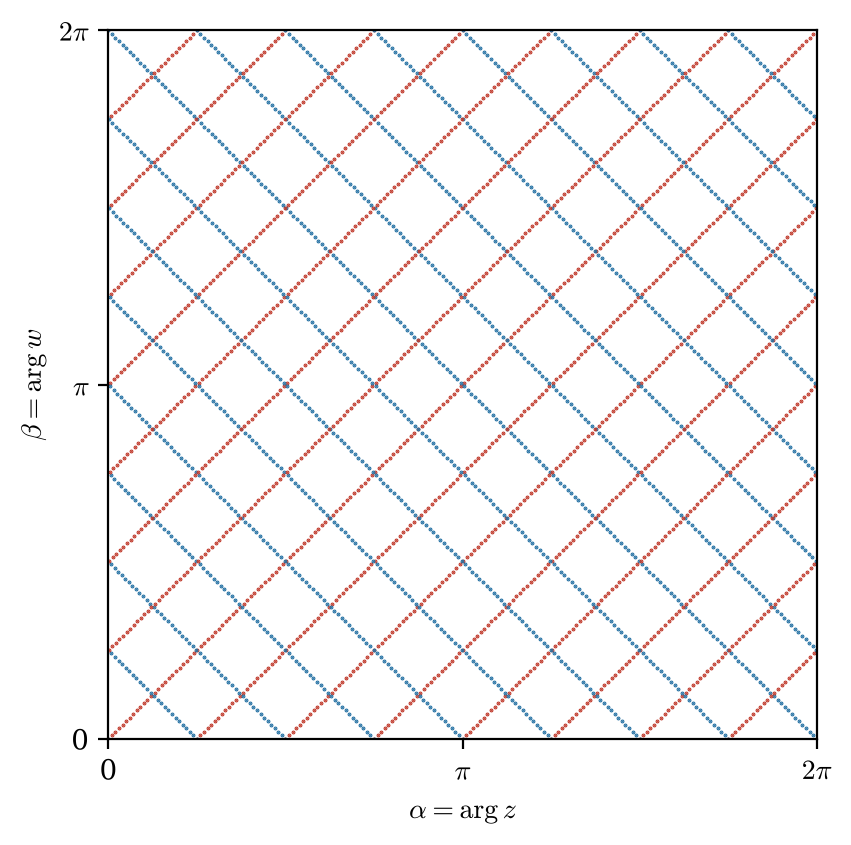
\includegraphics[width=0.9\textwidth]{fig_clifford.png}
\caption{The flat torus $T_{a,b}$ unrolled in arc-length coordinates, for $a=0.6$, $b=0.8$. The Hopf fibres are the lines of slope $b/a$ (solid), and the fibres of $(z,w)\mapsto h(\bar z,w)$ are the lines of slope $-b/a$ (dashed). After stereographic projection the two families become the two families of Villarceau circles (Chapter~\ref{ch:villarceau}).}
\label{fig:clifford}
\end{figure}

\begin{figure}[ht]
\centering
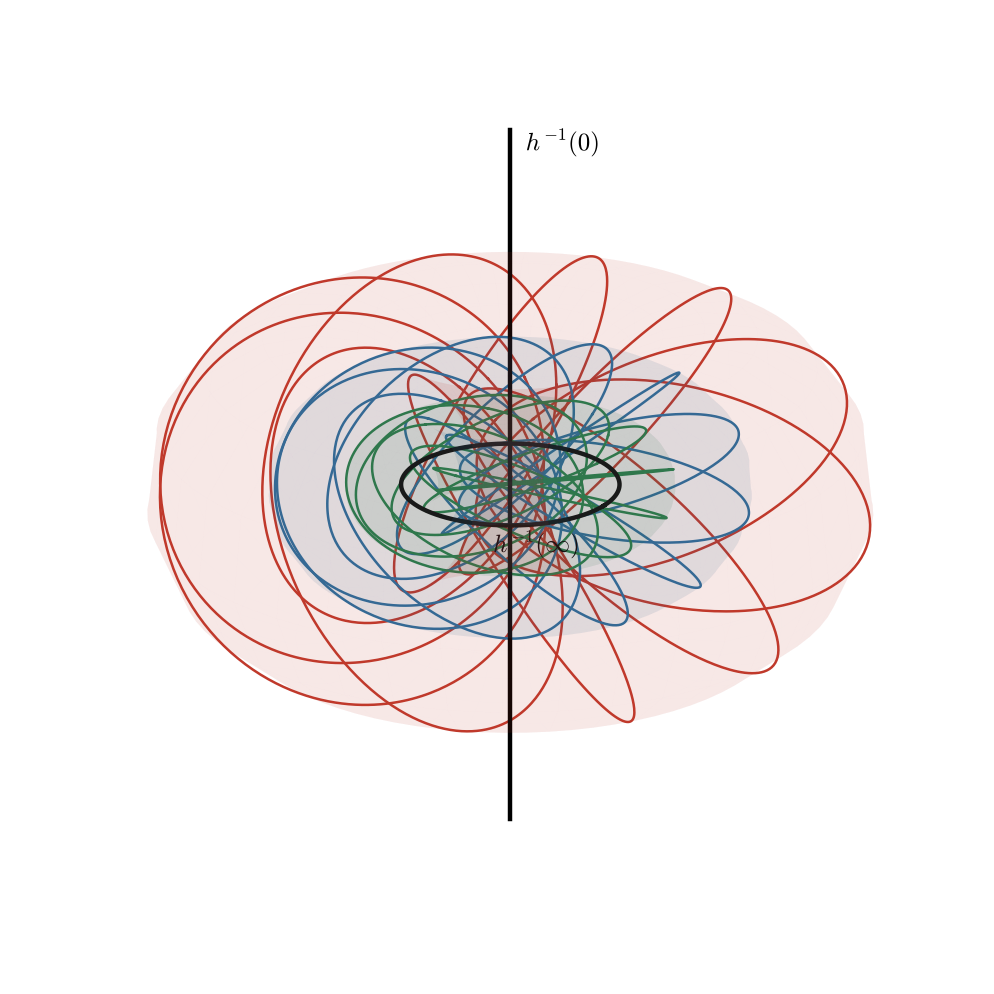
\includegraphics[width=0.85\textwidth]{fig_hopf_tori.png}
\caption{Nested tori $T_{a,b}$ in $\R^3$ after stereographic projection, each with some of its Hopf fibres; the vertical axis together with $\infty$ is the fibre over one pole, and the unit circle in the horizontal plane is the fibre over the other.}
\label{fig:hopftori}
\end{figure}

\section{The unit tangent bundle of the two-sphere}\label{sec:unittangent}

Identify $\R^3$ with $\Imag\Hq$ and $S^3$ with the unit quaternions. The map $\rho(q)(v)=qv\bar q$ is a surjective homomorphism $S^3\to\SO(3)$ with kernel $\{\pm1\}$ \cite[Section~2.3]{Bae02}, so $\SO(3)\cong S^3/\{\pm1\}=\RP^3$.

\begin{proposition}\label{prop:unittangent}
Let $T^1S^2=\{(p,v)\in S^2\times S^2:p\perp v\}$ be the unit tangent bundle. The map $\Psi\colon S^3\to T^1S^2$, $\Psi(q)=(qi\bar q,\,qj\bar q)$, is a two-fold covering that identifies $T^1S^2$ with $\RP^3$. Its composite with the projection to $S^2$ is $h'(q)=qi\bar q$, which is the Hopf map up to isometries of $S^3$ and of $S^2$, and the circle bundle $T^1S^2\to S^2$ is the quotient of the Hopf bundle by the antipodal action $q\mapsto-q$ on its fibres.
\end{proposition}

\begin{proof}
A point $(p,v)$ of $T^1S^2$ determines the positive orthonormal frame $(p,v,p\times v)$, and $\SO(3)$ acts simply transitively on such frames, so $(p,v)\mapsto$ the rotation taking $(i,j,k)$ to the frame is a diffeomorphism $T^1S^2\cong\SO(3)$, and $\Psi$ corresponds to $\rho$. For $q=z+wj$ with $z,w\in\C$ a direct computation, using $ji=-ij$ and $wj=j\bar w$, gives
\[
qi\bar q=(|z|^2-|w|^2)\,i+2\Imag(zw)\,j-2\Re(zw)\,k,
\]
which is $h(z,\bar w)=(2zw,|z|^2-|w|^2)$ followed by a linear isometry of $\R^3$. The fibres of $h'$ are the circles $\{qe^{i\theta}\}$, and $\Psi(qe^{i\theta})=(qi\bar q,\,qe^{2i\theta}j\bar q)$, so as $\theta$ runs over $[0,\pi]$ the tangent vector turns once around $p=qi\bar q$; the points $q$ and $-q$ of a fibre of $h'$ give the same point of $T^1S^2$.
\end{proof}

\begin{remark}
The Euler number of the Hopf bundle is $\pm1$ and that of $T^1S^2\to S^2$ is $\chi(S^2)=2$, in accordance with the quotient by $\pm1$, which doubles the Euler class of an oriented circle bundle. The total space of $T^1S^2$ is $\RP^3$, not $S^3$; its fundamental group is $\Z/2$, while $S^3$ is simply connected. Theorem~\ref{thm:F} follows from Propositions~\ref{prop:parallel}, \ref{prop:clifford} and \ref{prop:unittangent}.
\end{remark}

\chapter{Villarceau circles and Villarceau spheres}\label{ch:villarceau}

This chapter proves Theorem~\ref{thm:E} and Villarceau's theorem. The argument is the same for $d=2,4,8$: one fibre is computed explicitly, and the others are obtained from it by isometries that commute with stereographic projection. For octonions the only point that needs comment is that these isometries are left multiplications, which are orthogonal by \ref{D:norm}.

\section{Stereographic projection}\label{sec:stereo}

Fix $d\in\{2,4,8\}$ and a unit vector $\varepsilon\in\K$ with $\varepsilon\perp1$. For $v\in\K$ write $v_\varepsilon=\langle v,\varepsilon\rangle=\Re(v\bar\varepsilon)$ and $\pi(v)=v-v_\varepsilon\varepsilon\in\varepsilon^\perp$, the orthogonal projection onto the hyperplane $\varepsilon^\perp\subset\K$. Stereographic projection from the point $N=(0,\varepsilon)$ of $S^{2d-1}$ onto its tangent hyperplane at the antipode, translated to the origin, is
\begin{equation}\label{eq:sigmaN}
\sigma\colon S^{2d-1}\setminus\{N\}\to\K\times\varepsilon^\perp=\R^d\times\R^{d-1},\qquad
\sigma(A,B)=\frac{\bigl(A,\ \pi(B)\bigr)}{1-B_\varepsilon}.
\end{equation}
It is a conformal diffeomorphism, it maps round spheres not through $N$ to round spheres \cite{Lyo03}, and it commutes with every isometry of $\K^2$ that fixes $N$ and preserves the decomposition $\K\times\K$. For $d=2$ and $\varepsilon=i$,
\[
\sigma(z,w)=\frac{\bigl(z,\ \Re w\bigr)}{1-\Imag w}\in\C\times\R=\R^3 .
\]

For $0<a<1$ put $b=\sqrt{1-a^2}$ and $\Sigma_a=S^{d-1}(a)\times S^{d-1}(b)=\{(A,B):|A|=a,\ |B|=b\}\subset S^{2d-1}$. It does not contain $N$. Every point $(A,B)$ of $S^{2d-1}$ with $A\neq0\neq B$ lies on exactly one $\Sigma_a$, namely $a=|A|$, and $\Sigma_a=h_\K^{-1}\bigl(\{x_{d+1}=a^2-b^2\}\bigr)$ is the preimage of a sphere of latitude.

\begin{lemma}\label{lem:tube}
Let $R=1/a$ and $r=b/a$, so that $R^2-r^2=1$. Then $\sigma$ maps $\Sigma_a$ diffeomorphically onto the tube
\[
T_{R,r}=\bigl\{(x,y)\in\R^d\times\R^{d-1}:(|x|-R)^2+|y|^2=r^2\bigr\}.
\]
\end{lemma}

\begin{proof}
Let $(A,B)\in\Sigma_a$ and $\beta=B_\varepsilon\in[-b,b]$, so $|\pi(B)|^2=b^2-\beta^2$. For $(x,y)=\sigma(A,B)$ we have $|x|=a/(1-\beta)$ and $|y|^2=(b^2-\beta^2)/(1-\beta)^2$, hence
\[
a^2(1-\beta)^2\bigl((|x|-R)^2+|y|^2\bigr)=\bigl(a^2-(1-\beta)\bigr)^2+a^2(b^2-\beta^2)=(\beta-b^2)^2+a^2b^2-a^2\beta^2=b^2(1-\beta)^2,
\]
using $a^2-1=-b^2$ and $a^2+b^2=1$. So $(|x|-R)^2+|y|^2=b^2/a^2=r^2$. The restriction of $\sigma$ to $\Sigma_a$ is an injective immersion between compact connected manifolds of the same dimension $2d-2$, so it is a diffeomorphism onto $T_{R,r}$ by invariance of domain.
\end{proof}

For $d=2$, $T_{R,r}$ is the torus obtained by rotating the circle $(x_1-R)^2+x_3^2=r^2$ of the $(x_1,x_3)$-plane about the $x_3$-axis, a ring torus because $R>r$. For $d=4,8$ it is the boundary of the tubular neighbourhood of radius $r$ of the round sphere $S^{d-1}(R)\subset\R^d\times0$, diffeomorphic to $S^{d-1}\times S^{d-1}$.

\section{The fibres on a product of spheres}\label{sec:villfibres}

By Corollary~\ref{cor:fibration} the fibres of $h_\K$ contained in $\Sigma_a$ are those over the points $s(x)$ with $|x|=a/b$. Writing $x=(a/b)u$ with $|u|=1$ and $c=bc'$, the fibre over $s(x)$ is
\begin{equation}\label{eq:Fu}
F_u=\bigl\{\bigl(a\,(uc'),\ b\,c'\bigr):|c'|=1\bigr\},\qquad u\in S^{d-1},
\end{equation}
where we used $((a/b)u)(bc')=a(uc')$, valid because $a,b$ are real. In particular $F_1=\{(ac,bc):|c|=1\}$.

\begin{proposition}[The base fibre]\label{prop:basefibre}
Let $\Pi_1=\{(x,\,r\,\pi(x)):x\in\K\}\subset\R^d\times\R^{d-1}$, a $d$-dimensional linear subspace. Then $\sigma(F_1)$ is the round $(d-1)$-sphere in $\Pi_1$ with centre $(r\varepsilon,0)$ and radius $R$.
\end{proposition}

\begin{proof}
For $c\in S^{d-1}$ put $t=c_\varepsilon$. Then $\sigma(ac,bc)=(x,y)$ with $x=ac/(1-bt)$ and $y=b\pi(c)/(1-bt)=(b/a)\pi(x)$, so $\sigma(F_1)\subset\Pi_1$. For $\rho\in\R$,
\[
(1-bt)^2\bigl(|x-\rho\varepsilon|^2+|y|^2\bigr)=a^2-2a\rho t(1-bt)+\rho^2(1-bt)^2+b^2(1-t^2),
\]
and for $\rho=r=b/a$ the right-hand side equals $(1+r^2)(1-bt)^2$, as one checks by comparing the coefficients of $1$, $t$ and $t^2$:
\[
1+r^2,\qquad -2a\rho-2b\rho^2=-2b(1+r^2),\qquad -b^2+2ab\rho+b^2\rho^2=b^2(1+r^2).
\]
Hence $|x-r\varepsilon|^2+|y|^2=1+r^2=R^2$. The centre $(r\varepsilon,0)$ lies in $\Pi_1$, since $\pi(\varepsilon)=0$. So $\sigma(F_1)$ lies on the round $(d-1)$-sphere $S_1^+$ of $\Pi_1$ with this centre and radius, and it fills it, being a compact $(d-1)$-manifold embedded in the connected $(d-1)$-manifold $S_1^+$.
\end{proof}

\begin{proof}[Proof of Theorem~\ref{thm:E}]
For $u\in S^{d-1}$ the map $\Lambda_u(A,B)=(uA,B)$ is an isometry of $\K^2$, since $\ell_u$ is orthogonal, and it fixes $N$ and preserves $\Sigma_a$. By \eqref{eq:sigmaN}, $\sigma\circ\Lambda_u=\lambda_u\circ\sigma$ with $\lambda_u(x,y)=(ux,y)$, an isometry of $\R^d\times\R^{d-1}$. By \eqref{eq:Fu}, $\Lambda_u(F_1)=\{(u(ac),bc)\}=F_u$, because $u(ac)=a(uc)$. Hence
\[
\sigma(F_u)=\lambda_u\bigl(\sigma(F_1)\bigr)
\]
is the round $(d-1)$-sphere of radius $R$ with centre $(ur\varepsilon,0)$, at distance $r$ from the origin, in the $d$-dimensional linear subspace $\Pi_u=\lambda_u(\Pi_1)$. The fibres $F_u$ partition $\Sigma_a$ by Proposition~\ref{prop:lines}, and $\sigma|_{\Sigma_a}$ is a bijection onto $T_{R,r}$ (Lemma~\ref{lem:tube}), so the spheres $\sigma(F_u)$ partition $T_{R,r}$. For $d=2$ the statements about the two families of Villarceau circles are proved in Section~\ref{sec:villarceau2} below.
\end{proof}

We call the spheres $\sigma(F_u)$ \emph{Villarceau spheres} of the tube. The next proposition shows that, as for circles on a torus, they come in two families and are cut out by linear subspaces tangent to the tube.

\begin{proposition}[Two families]\label{prop:twofamilies}
Let $\rho_\varepsilon(v)=v-2v_\varepsilon\varepsilon$ be the reflection of $\K$ in $\varepsilon^\perp$. Then:
\begin{enumerate}[label=\textup{(\roman*)}]
\item $\Pi_1\cap T_{R,r}=S_1^+\cup S_1^-$, where $S_1^\pm$ is the round $(d-1)$-sphere of $\Pi_1$ with centre $(\pm r\varepsilon,0)$ and radius $R$.
\item $S_1^-=\sigma(\rho_\varepsilon\times\mathrm{id})(F_1)$ is the image of a fibre of the map $h_\K\circ(\rho_\varepsilon\times\mathrm{id})$, whose fibres on $\Sigma_a$ also map onto Villarceau spheres partitioning $T_{R,r}$.
\item $S_1^+\cap S_1^-$ is the unit $(d-2)$-sphere $\{(x,rx):x\in\varepsilon^\perp,\ |x|=a\}$, and $\Pi_1$ is tangent to $T_{R,r}$ at each of its points.
\end{enumerate}
The same holds for $\Pi_u$, by applying $\lambda_u$.
\end{proposition}

\begin{proof}
(i) Write a point of $\Pi_1$ as $(x,r\pi(x))$ and put $\xi=x_\varepsilon$, $\eta=|\pi(x)|^2$, so $|x|^2=\xi^2+\eta$. Let $G_\pm=(\xi\mp r)^2+(1+r^2)\eta-(1+r^2)$ be the equations of $S_1^\pm$ in $\Pi_1$ (the squared distance from $(\pm r\varepsilon,0)$ is $(\xi\mp r)^2+\eta+r^2\eta$). With $\mathcal A=\xi^2+(1+r^2)\eta-1$ we have $G_\pm=\mathcal A\mp2r\xi$, so $G_+G_-=\mathcal A^2-4r^2\xi^2$. On the other hand, since $|x|+R>0$ and $|x|^2+1+r^2\eta>0$, the equation of the tube restricted to $\Pi_1$, $(|x|-R)^2+r^2\eta=r^2$, is equivalent to $(|x|^2+1+r^2\eta)^2=4R^2|x|^2$, that is to
\[
(\mathcal A+2)^2-4(1+r^2)(\xi^2+\eta)=0 .
\]
Expanding, $(\mathcal A+2)^2-4(1+r^2)(\xi^2+\eta)=\mathcal A^2-4r^2\xi^2+4\bigl(\mathcal A+1-\xi^2-(1+r^2)\eta\bigr)=G_+G_-$. So $\Pi_1\cap T_{R,r}=\{G_+G_-=0\}=S_1^+\cup S_1^-$.

(ii) $\rho_\varepsilon\times\mathrm{id}$ is an isometry of $\K^2$ fixing $N$ and preserving $\Sigma_a$, and $\sigma\circ(\rho_\varepsilon\times\mathrm{id})=(\rho_\varepsilon\times\mathrm{id})\circ\sigma$. Since $\pi\circ\rho_\varepsilon=\pi$, the isometry $\rho_\varepsilon\times\mathrm{id}$ of $\R^d\times\R^{d-1}$ preserves $\Pi_1$ and maps the centre $(r\varepsilon,0)$ to $(-r\varepsilon,0)$, so it maps $S_1^+$ to $S_1^-$. The second statement follows from Theorem~\ref{thm:E} by conjugating with $\rho_\varepsilon\times\mathrm{id}$.

(iii) $G_+=G_-=0$ forces $\xi=0$ and then $\eta=1/(1+r^2)=a^2$; the points are $(x,rx)$ with $x\in\varepsilon^\perp$, $|x|=a$, and $|(x,rx)|^2=a^2(1+r^2)=1$. At such a point $p$ the two spheres $S_1^\pm$ meet transversally inside $\Pi_1$, because $p$ is not on the line through their centres ($\xi=0$ and $\eta\neq0$), so $T_pS_1^++T_pS_1^-=\Pi_1$. Both tangent spaces lie in $T_pT_{R,r}$, hence $\Pi_1\subset T_pT_{R,r}$.
\end{proof}

For $d=2$ the reflection $\rho_\varepsilon$ with $\varepsilon=i$ is complex conjugation, and the second family consists of the fibres of $(z,w)\mapsto h(\bar z,w)$. For $d=4,8$ the two families are the fibres of $h_\K$ and of $h_\K\circ(\rho_\varepsilon\times\mathrm{id})$ on $\Sigma_a$; the subspaces $\Pi_u$ play the role of the bitangent planes, being tangent to the tube along a unit $(d-2)$-sphere.

\section{Villarceau's theorem}\label{sec:villarceau2}

Now let $d=2$, $\varepsilon=i$, and coordinates $(x_1,x_2,x_3)$ on $\R^3=\C\times\R$. Then $\pi(x)=x_1$, the plane $\Pi_1$ is $\{x_3=r\,x_1\}$, and the circles $S_1^\pm$ have centres $(0,\pm r,0)$ and radius $R$.

\begin{proposition}\label{prop:bitangent}
Let $T=T_{R,r}$ with $R>r>0$, not necessarily with $R^2-r^2=1$, and let $\phi\in(0,\pi/2)$ be defined by $\sin\phi=r/R$. The planes through the centre of $T$ that are tangent to $T$ are exactly the planes obtained from
\[
\Pi=\{x_3=x_1\tan\phi\}
\]
by rotation about the $x_3$-axis. Each of them is tangent to $T$ at two antipodal points, at distance $\sqrt{R^2-r^2}$ from the centre, and meets $T$ in the two circles of radius $R$ with centres $(0,\pm r,0)$ in the case of $\Pi$.
\end{proposition}

\begin{proof}
Let $\Pi'$ be a plane through $0$ tangent to $T$ at $p$. After a rotation about the axis, $p$ lies in the half-plane $\{x_2=0,\ x_1>0\}$, on the meridian circle $M=\{(x_1-R)^2+x_3^2=r^2\}$. The tangent plane $T_pT$ is spanned by $e_2$, the direction of the parallel through $p$, and the tangent line of $M$ at $p$. As $\Pi'=p+T_pT$ contains $0$ and $p$, its intersection with the plane $x_2=0$ is the line through $0$ and $p$, and it is also the tangent line of $M$ at $p$. The tangent lines of $M$ through the origin are $x_3=\pm x_1\tan\phi$, because the distance from the centre $(R,0)$ of $M$ to such a line is $R\sin\phi=r$. Their points of tangency are $(R\cos^2\phi,\pm R\cos\phi\sin\phi)$, at distance $R\cos\phi=\sqrt{R^2-r^2}$ from $0$. The plane $\{x_3=-x_1\tan\phi\}$ is the image of $\Pi$ under the rotation by $\pi$ about the axis, so $\Pi'$ is a rotation of $\Pi$. Conversely $\Pi$ contains $e_2$ and the tangent line of $M$ at $(R\cos^2\phi,0,R\cos\phi\sin\phi)$, so it is tangent to $T$ there, and by the symmetry $x\mapsto-x$ of $T$ also at the antipodal point.

For the intersection use the coordinates $(\upsilon,v)$ on $\Pi$, where $x=(\upsilon\cos\phi,\ v,\ \upsilon\sin\phi)$. The torus is $\{(|x|^2+R^2-r^2)^2=4R^2(x_1^2+x_2^2)\}$, and on $\Pi$, with $s=\upsilon^2+v^2$,
\[
(s+R^2-r^2)^2-4R^2(\upsilon^2\cos^2\phi+v^2)
=\bigl(\upsilon^2+(v-r)^2-R^2\bigr)\bigl(\upsilon^2+(v+r)^2-R^2\bigr)+4\upsilon^2\bigl(R^2\sin^2\phi-r^2\bigr),
\]
an identity of polynomials (Appendix~\ref{app:villarceau}). The last term vanishes because $\sin\phi=r/R$. So $\Pi\cap T$ is the union of the circles $\upsilon^2+(v\mp r)^2=R^2$, whose centres are the points $(0,\pm r,0)$.
\end{proof}

\begin{proof}[Proof of Corollary~\ref{cor:intro-villarceau}]
Let $T$ be a ring torus with radii $R>r>0$, and let $\mu=\sqrt{R^2-r^2}$. The similarity $x\mapsto x/\mu$ maps $T$ to $T_{R',r'}$ with $R'=R/\mu$, $r'=r/\mu$ and $R'^2-r'^2=1$, and it maps planes through the centre tangent to $T$ to planes through the centre tangent to $T_{R',r'}$. Put $a=1/R'$ and $b=r'/R'$; then $a^2+b^2=(1+r'^2)/R'^2=1$. By Theorem~\ref{thm:E} and Proposition~\ref{prop:twofamilies}, the plane $\Pi_1=\{x_3=r'x_1\}$ meets $T_{R',r'}$ in $\sigma(F_1)$ and in its mirror image, the image of a fibre of $h(\bar z,w)$. Here $\tan\phi=r'$ is equivalent to $\sin\phi=r'/R'$ because $R'^2=1+r'^2$, so $\Pi_1$ is the plane $\Pi$ of Proposition~\ref{prop:bitangent}. Every other plane through the centre tangent to $T_{R',r'}$ is $\lambda_u(\Pi_1)$ for a rotation $\lambda_u$ about the axis, and meets $T_{R',r'}$ in $\sigma(F_u)$ and its mirror image. Scaling back by $\mu$ proves the corollary; the circles have radius $\mu R'=R$.
\end{proof}

\begin{remark}
Villarceau's original statement \cite{Vil48} is that the bitangent plane cuts the torus in two circles. Proposition~\ref{prop:bitangent} proves it directly, and the Hopf fibration explains it: each circle is a great circle of $S^3$ lying on a flat torus $T_{a,b}$, and stereographic projection maps circles to circles. The geodesics of slope $\pm b/a$ on $T_{a,b}$ (Proposition~\ref{prop:clifford}) become the two families of Villarceau circles; the meridians and parallels are the images of the coordinate circles $\alpha=\mathrm{const}$ and $\beta=\mathrm{const}$. The Villarceau circles are not the curves $\theta\pm\varphi=\mathrm{const}$ in the usual angular coordinates $(R+r\cos\theta)(\cos\varphi,\sin\varphi)$, $r\sin\theta$ of the torus, which are not circles; they are the curves $\beta\mp\alpha=\mathrm{const}$ in the coordinates of $T_{a,b}$, which differ from the usual angles by a conformal reparametrisation of the meridian.\footnote{Stereographic projection maps the meridian circle $\{\alpha=\alpha_0\}$ of $T_{a,b}$ onto the meridian of the image torus, but not with constant speed: the angle $\beta$ on $T_{a,b}$ and the angle $\theta$ about the centre of the meridian are related by a M\"obius transformation of the circle.}
\end{remark}

\begin{figure}[ht]
\centering
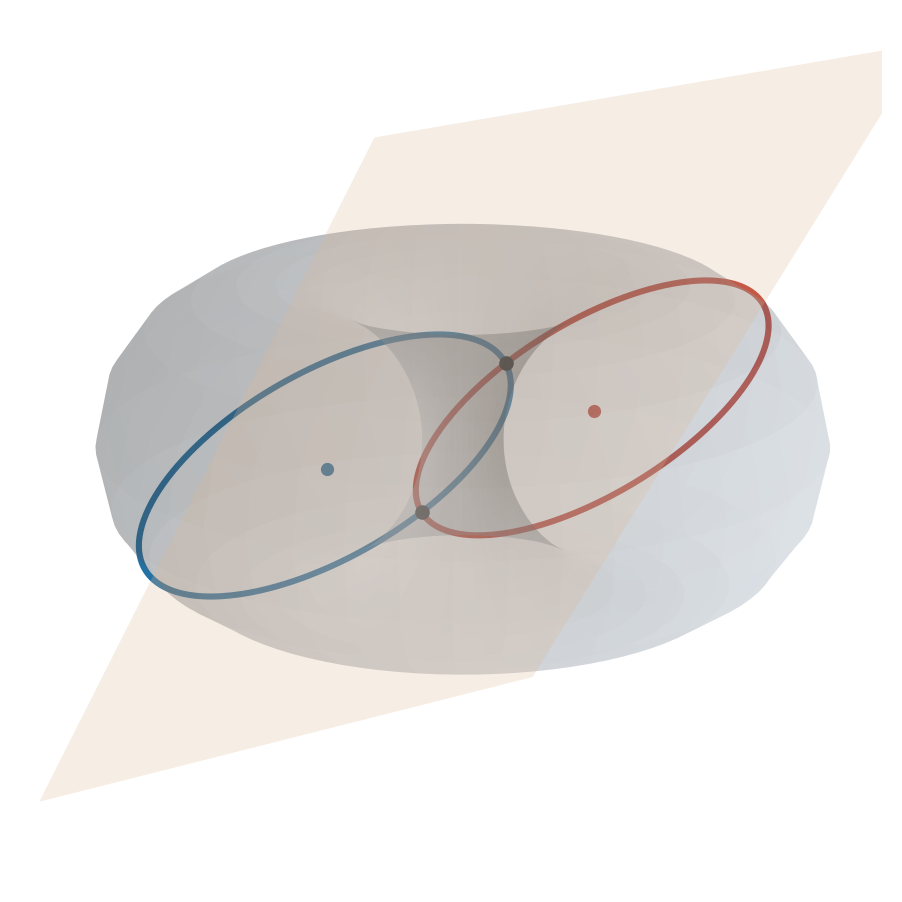
\includegraphics[width=0.92\textwidth]{fig_villarceau.png}
\caption{A ring torus with $R^2-r^2=1$, the bitangent plane $\Pi$ through its centre, the two Villarceau circles $\sigma(F_1)$ and its mirror image, of radius $R$ and centres $(0,\pm r,0)$, and the two points of tangency at distance $1$ from the centre.}
\label{fig:villarceau}
\end{figure}

\section{The meridians are Apollonian circles}\label{sec:apollonius}

As $a$ varies in $(0,1)$ the tori $T_{R,r}=\sigma(\Sigma_a)$ fill $\R^3$ minus the $x_3$-axis and the unit circle of the horizontal plane, which are the images of the fibres over the two poles. Their meridians in the half-plane $\{x_2=0,\ x_1>0\}$ are the circles
\[
M_R=\{(x_1-R)^2+x_3^2=R^2-1\},\qquad R>1 .
\]

\begin{proposition}\label{prop:apollonius}
$M_R$ is the circle of Apollonius $\{P:|P-(1,0)|=\kappa\,|P-(-1,0)|\}$ with $\kappa^2=(R-1)/(R+1)=(1-a)/(1+a)$. The circles $M_R$ form the hyperbolic pencil of circles with limit points $(\pm1,0)$, and they are orthogonal to every circle through $(1,0)$ and $(-1,0)$.
\end{proposition}

\begin{proof}
On $M_R$ we have $x_1^2+x_3^2=2Rx_1-1$, so $|P-(1,0)|^2=2(R-1)x_1$ and $|P-(-1,0)|^2=2(R+1)x_1$. The ratio is $(R-1)/(R+1)$, and $R=1/a$ gives the second expression. For the orthogonality, an inversion centred at $(-1,0)$ maps the circles $M_R$ to concentric circles about the image of $(1,0)$, and the circles through $(\pm1,0)$ to lines through that point; inversions preserve angles.
\end{proof}

The limit point $(1,0)$ is the point of the meridian half-plane on the unit circle, the image of the fibre over one pole, and the tori shrink to it as $a\to1$; as $a\to0$ they grow towards the axis. Figure~\ref{fig:meridians} shows the pencil together with the bitangent lines of one meridian.

\begin{figure}[ht]
\centering
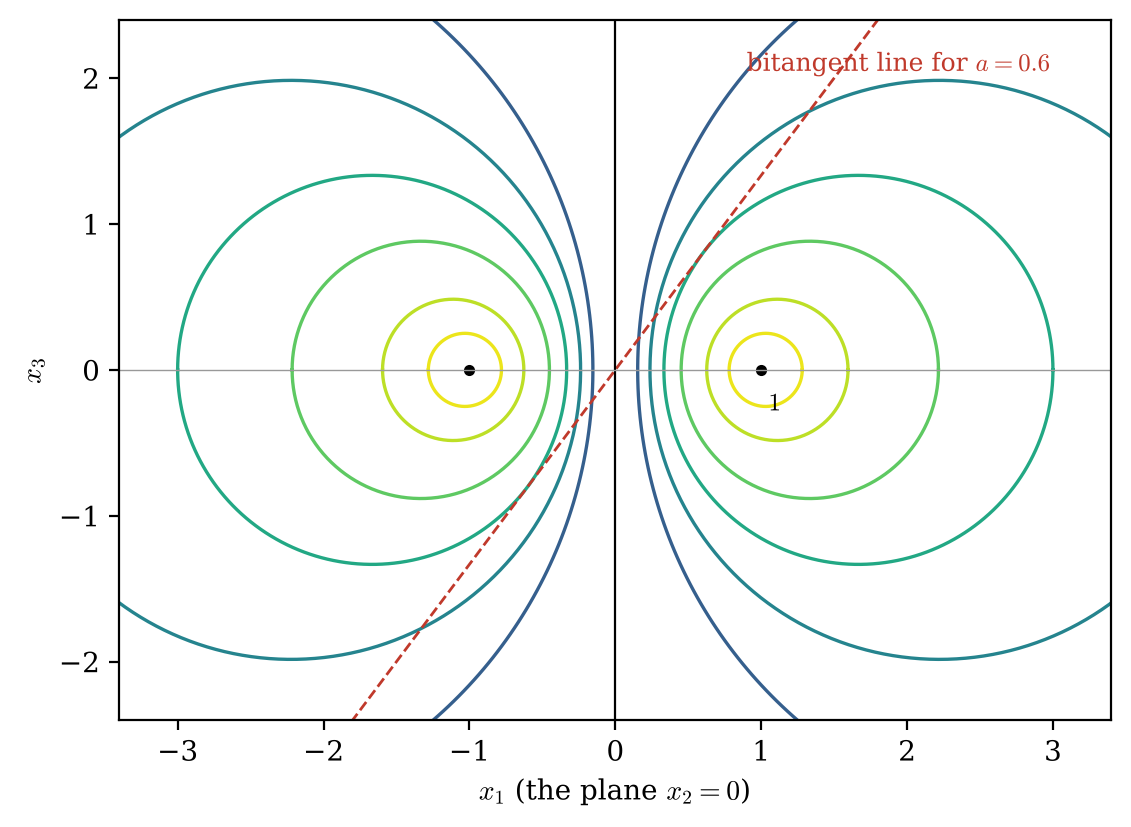
\includegraphics[width=0.8\textwidth]{fig_meridians.png}
\caption{Meridians of the tori $\sigma(\Sigma_a)$ in the half-plane $x_2=0$: the Apollonian circles with limit points $(\pm1,0)$. The line through the origin tangent to one meridian is the trace of a bitangent plane, and its point of tangency lies on the unit circle.}
\label{fig:meridians}
\end{figure}

The point of tangency of every bitangent plane lies at distance $\sqrt{R^2-r^2}=1$ from the centre, by Proposition~\ref{prop:bitangent}. So in the meridian half-plane the points of tangency of all the tori $\sigma(\Sigma_a)$ lie on the unit circle, which is the circle through the two limit points orthogonal to all the meridians; in higher dimensions Proposition~\ref{prop:twofamilies}(iii) gives the same statement with the unit $(d-2)$-sphere.

\chapter{Stable stems, the image of \texorpdfstring{$J$}{J} and the Kervaire invariant}\label{ch:stable}

This chapter surveys what is known about the stable stems in the range where the Hopf maps are visible. Nothing here is new; the purpose is to state the results precisely, with their sources, and to separate the proved from the announced. Section~\ref{sec:parallel} contains the one elementary proof of the chapter.

\section{The stable stems through dimension nineteen}\label{sec:stems}

By Theorem~\ref{thm:freudenthal}, $\pi_k^s=\pi_{n+k}(S^n)$ for $n\ge k+2$. Table~\ref{tab:stable} lists $\pi_k^s$ for $k\le19$, after Toda \cite{Tod62} and Ravenel \cite[Table~A3.3]{Rav86}; the computations have since been extended far beyond this range by Isaksen, Wang and Xu \cite{IWX23}.

\begin{table}[ht]
\centering
\small
\begin{tabular}{@{}c|cccccccccc@{}}
\toprule
$k$ & $0$ & $1$ & $2$ & $3$ & $4$ & $5$ & $6$ & $7$ & $8$ & $9$\\
$\pi_k^s$ & $\Z$ & $2$ & $2$ & $24$ & $0$ & $0$ & $2$ & $240$ & $2^2$ & $2^3$\\
\midrule
$k$ & $10$ & $11$ & $12$ & $13$ & $14$ & $15$ & $16$ & $17$ & $18$ & $19$\\
$\pi_k^s$ & $6$ & $504$ & $0$ & $3$ & $2^2$ & $480{\oplus}2$ & $2^2$ & $2^4$ & $8{\oplus}2$ & $264{\oplus}2$\\
\bottomrule
\end{tabular}
\caption{The stable stems $\pi_k^s$ for $k\le19$ \cite{Tod62}, \cite[Table~A3.3]{Rav86}; an integer $m$ stands for $\Z/m$ and $2^j$ for $(\Z/2)^j$.}
\label{tab:stable}
\end{table}

The groups in degrees $1$, $3$ and $7$ are generated by the suspensions $\eta$, $\nu$, $\sigma$ of the three Hopf maps, and in degrees $2$, $6$ and $14$ the squares $\eta^2$, $\nu^2$ and $\sigma^2$ are nonzero \cite{Tod62}. The cyclic summands of orders $24$, $240$, $504$, $480$ and $264$ in degrees $3,7,11,15,19$ form the image of the $J$-homomorphism, described next.

\section{The \texorpdfstring{$J$}{J}-homomorphism}\label{sec:J}

An element of $\pi_k(\SO(n))$, represented by $\alpha\colon S^k\to\SO(n)$, defines a map $S^k\times S^{n-1}\to S^{n-1}$, $(x,v)\mapsto\alpha(x)v$, and the Hopf construction turns it into a map $S^{k+n}=S^k*S^{n-1}\to\Sigma S^{n-1}=S^n$. This defines Whitehead's homomorphism $J\colon\pi_k(\SO(n))\to\pi_{n+k}(S^n)$ \cite{Whi42}, compatible with suspension, and in the limit the stable homomorphism
\[
J\colon\pi_k(\SO)\to\pi_k^s .
\]
For $\K=\C,\Hq,\Oc$ the multiplication of unit vectors $S^{d-1}\times S^{d-1}\to S^{d-1}$ is the map associated with the clutching function $\tau$ of \eqref{eq:clutch}, and its Hopf construction is, up to homotopy and sign, the Hopf map $h_\K$; this is the classical link between the Hopf maps and $J$.

By Bott periodicity \cite{Bot59}, $\pi_k(\SO)$ for $k\ge1$ depends only on $k\bmod8$:
\[
\begin{array}{c|cccccccc}
k\bmod 8 & 0&1&2&3&4&5&6&7\\\hline
\pi_k(\SO) & \Z/2&\Z/2&0&\Z&0&0&0&\Z
\end{array}
\]

\begin{theorem}[Adams, Quillen, Sullivan, Becker--Gottlieb]\label{thm:imJ}
For $k\ge1$ the image of $J$ in $\pi_{4k-1}^s$ is a cyclic direct summand whose order is the denominator of $B_{2k}/4k$, where $B_{2k}$ is the Bernoulli number. For $k\ge1$ the image of $J$ in $\pi_{8k}^s$ and in $\pi_{8k+1}^s$ is $\Z/2$, and $J$ is injective on $\pi_{8k}(\SO)$ and $\pi_{8k+1}(\SO)$.
\end{theorem}

Adams \cite{Ada66} proved the lower bounds and the upper bound for the odd part, and reduced the rest to the \emph{Adams conjecture}: for a real vector bundle $\xi$ over a finite CW complex $X$ and an integer $\ell$, there is $e\ge0$ such that $\ell^e(\psi^\ell\xi-\xi)$ is fibre homotopy trivial, that is, maps to zero in $J(X)$, where $\psi^\ell$ is the Adams operation. The conjecture was proved by Quillen \cite{Qui71}, by Sullivan \cite{Sul74}, and by Becker and Gottlieb \cite{BG75}.\footnote{The statement of the conjecture in the earlier version of this work was garbled; the formulation here is that of \cite{Ada66}.}

\begin{table}[ht]
\centering
\small
\begin{tabular}{@{}c|cccccccccc@{}}
\toprule
$k$ & $1$ & $2$ & $3$ & $4$ & $5$ & $6$ & $7$ & $8$ & $9$ & $10$\\
\midrule
stem $4k-1$ & $3$ & $7$ & $11$ & $15$ & $19$ & $23$ & $27$ & $31$ & $35$ & $39$\\
$B_{2k}$ & $\frac16$ & $-\frac1{30}$ & $\frac1{42}$ & $-\frac1{30}$ & $\frac5{66}$ & $-\frac{691}{2730}$ & $\frac76$ & $-\frac{3617}{510}$ & $\frac{43867}{798}$ & $-\frac{174611}{330}$\\
$|\im J|$ & $24$ & $240$ & $504$ & $480$ & $264$ & $65520$ & $24$ & $16320$ & $28728$ & $13200$\\
\bottomrule
\end{tabular}
\caption{The order of the image of $J$ in $\pi_{4k-1}^s$, the denominator of $B_{2k}/4k$ (Theorem~\ref{thm:imJ}); the values are recomputed in Appendix~\ref{app:checks}.}
\label{tab:imJ}
\end{table}

\begin{remark}\label{rem:vonstaudt}
Write $m(2k)$ for the denominator of $B_{2k}/4k$. By the von Staudt--Clausen theorem the denominator of $B_{2k}$ is the product of the primes $p$ with $(p-1)\mid2k$, and for the other primes $B_{2k}/2k$ is $p$-integral (a consequence of the Kummer congruences). Hence
\[
m(2k)=2^{\,2+\nu_2(2k)}\prod_{p\ \mathrm{odd},\ (p-1)\mid 2k}p^{\,1+\nu_p(2k)},
\]
which gives $m(2)=2^3\cdot3=24$, $m(4)=2^4\cdot3\cdot5=240$, $m(6)=2^3\cdot3^2\cdot7=504$, $m(12)=2^4\cdot3^2\cdot5\cdot7\cdot13=65520$ and $m(14)=2^3\cdot3=24$. The formula is checked against Table~\ref{tab:imJ}, and against the Bernoulli numbers for $k\le60$, in Appendix~\ref{app:checks}.
\end{remark}

Figure~\ref{fig:imJ} shows the orders on a logarithmic scale.

\begin{figure}[ht]
\centering
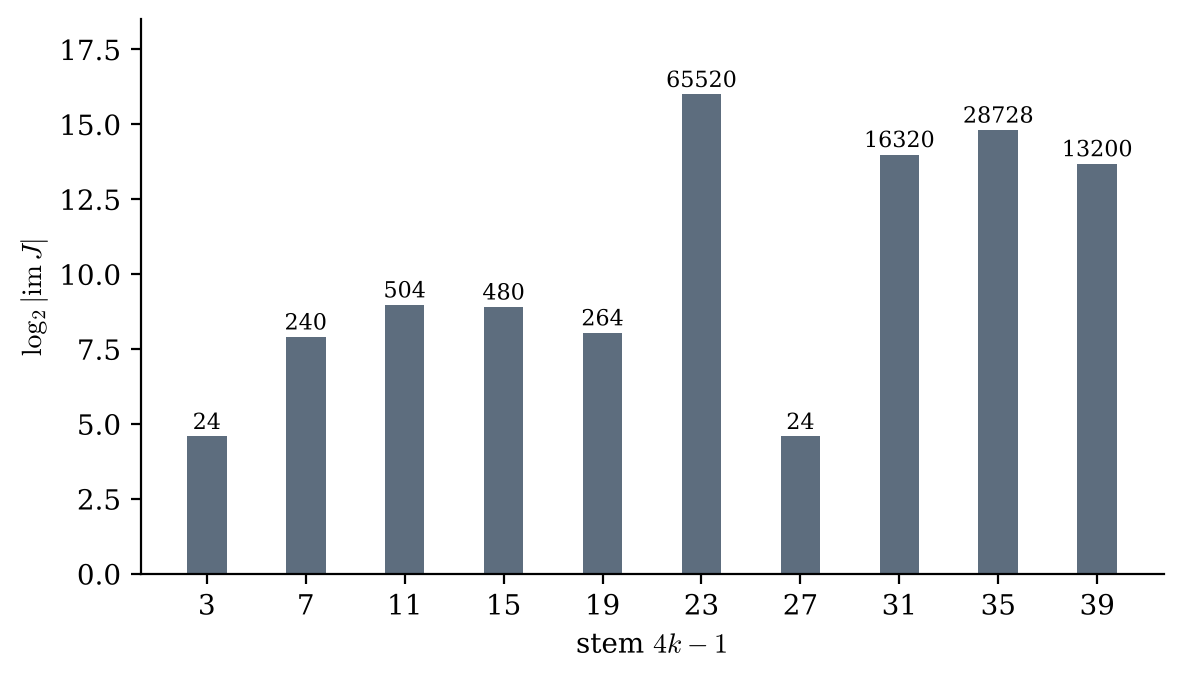
\includegraphics[width=0.85\textwidth]{fig_imageJ.png}
\caption{$\log_2|\im J|$ in the stems $4k-1$, $k=1,\dots,10$. The order is $24$ for $k=1$ and $k=7$, when $2$ and $3$ are the only primes $p$ with $(p-1)\mid2k$, and it is large when many such primes occur, as for $k=6$ (the primes $2,3,5,7,13$).}
\label{fig:imJ}
\end{figure}

\section{Division algebras and parallelisable spheres}\label{sec:parallel}

\begin{proposition}\label{prop:parallelisable}
The spheres $S^1$, $S^3$ and $S^7$ are parallelisable: if $e_1,\dots,e_{d-1}$ is an orthonormal basis of $\Imag\K$, then $x\mapsto xe_j$, $j=1,\dots,d-1$, are $d-1$ vector fields on $S^{d-1}$ that are orthonormal at every point.
\end{proposition}

\begin{proof}
By \ref{D:inner} and Lemma~\ref{lem:artin}, $\langle xa,xb\rangle=\langle a,\bar x(xb)\rangle=|x|^2\langle a,b\rangle$. For $|x|=1$ this gives $\langle xe_j,xe_k\rangle=\delta_{jk}$ and $\langle xe_j,x\rangle=\langle e_j,1\rangle=0$, so the vectors $xe_j$ are tangent to $S^{d-1}$ at $x$ and orthonormal.
\end{proof}

The converse is deep: $S^{n-1}$ is parallelisable only for $n=1,2,4,8$, by Bott--Milnor \cite{BM58} and Kervaire, and Adams determined the maximal number of linearly independent vector fields on every sphere \cite{Ada62}. Together with Corollary~\ref{cor:spherebundles} and Adams' theorem (I4), this is the topological form of the statement that $\R,\C,\Hq,\Oc$ are the only real normed division algebras.

\section{The Kervaire invariant}\label{sec:kervaire}

A framed manifold of dimension $4j+2$ has a Kervaire invariant in $\Z/2$, the Arf invariant of a quadratic refinement of its intersection form on middle-dimensional homology with $\Z/2$ coefficients; through the Pontryagin--Thom construction it becomes a homomorphism $\pi_{4j+2}^s\to\Z/2$. Browder proved that it vanishes unless the dimension has the form $2^{j+1}-2$ \cite{Bro69}. Let $\theta_j$ denote an element of Kervaire invariant one in $\pi_{2^{j+1}-2}^s$, when one exists.

\begin{theorem}\label{thm:kervaire}
\begin{enumerate}[label=\textup{(\roman*)}]
\item Elements $\theta_j$ exist for $j=1,2,3$, namely $\eta^2$, $\nu^2$ and $\sigma^2$, in the stems $2$, $6$ and $14$; for $j=4$ in stem $30$ \cite{BMT70}; and for $j=5$ in stem $62$ \cite{BJM84}.
\item No element $\theta_j$ exists for $j\ge7$, that is in the stems $254,510,\dots$ \cite{HHR16}.
\end{enumerate}
\end{theorem}

The only remaining case is $j=6$, the stem $126$. Lin, Wang and Xu \cite{LWX24} have announced a proof that $\theta_6$ exists; at the time of writing this is a preprint, and we record it as such. The first three cases show that the Hopf maps of the three non-commutative division algebras produce, through their squares, the first three elements of Kervaire invariant one.

\begin{remark}
Theorem~\ref{thm:kervaire} has a geometric meaning: for $j\neq6$ there is a closed smooth framed manifold of dimension $2^{j+1}-2$ with Kervaire invariant one exactly when $j\le5$ \cite{Bro69}, \cite{HHR16}.
\end{remark}

\chapter{Torus fibrations, Calabi--Yau geometry and exotic spheres}\label{ch:cy}

The Hopf fibration is the simplest example of several structures that appear in geometry and physics. This chapter states three of them precisely and proves what is elementary: the Clifford tori are special Lagrangian (Section~\ref{sec:syz}), the O'Neill tensor of the Hopf submersions is determined by Theorem~\ref{thm:F} (Section~\ref{sec:oneill}), and the quaternionic Hopf bundle is the first member of Milnor's family of $S^3$-bundles over $S^4$ (Section~\ref{sec:milnor}).

\section{Special Lagrangian tori and the SYZ picture}\label{sec:syz}

Let $X$ be a Calabi--Yau manifold of complex dimension $n$, with K\"ahler form $\omega$ and holomorphic volume form $\Omega$, with $\omega^n$ a constant multiple of $i^{n^2}\Omega\wedge\bar\Omega$. A real $n$-dimensional submanifold $L$ is \emph{special Lagrangian} of phase $\theta$ if $\omega|_L=0$ and $\Imag(e^{-i\theta}\Omega)|_L=0$. The conjecture of Strominger, Yau and Zaslow \cite{SYZ96} proposes that a Calabi--Yau manifold near a large complex structure limit admits a fibration by special Lagrangian $n$-tori, possibly with singular fibres, and that its mirror is obtained by dualising the tori. The conjecture concerns the existence of such a fibration; it does not prescribe the base.\footnote{For a simply connected Calabi--Yau threefold the base is expected to be a homology $3$-sphere, and Gross constructed topological $T^3$-fibrations of the quintic threefold and its mirror over $S^3$ \cite{Gro01}. This is a theorem about topological fibrations; the existence of special Lagrangian fibrations of compact Calabi--Yau threefolds remains open in general.}

The model case is the flat Calabi--Yau surface $(\C^*)^2$ with
\[
\omega_0=\frac i2\Bigl(\frac{dz\wedge d\bar z}{|z|^2}+\frac{dw\wedge d\bar w}{|w|^2}\Bigr),\qquad \Omega_0=\frac{dz}{z}\wedge\frac{dw}{w},
\]
which in the coordinates $z=e^{s_1+i\alpha}$, $w=e^{s_2+i\beta}$ are $\omega_0=ds_1\wedge d\alpha+ds_2\wedge d\beta$ and $\Omega_0=(ds_1+i\,d\alpha)\wedge(ds_2+i\,d\beta)$. This is $(\R\times S^1)^2$ with its flat metric.

\begin{proposition}\label{prop:slag}
The fibres of $\operatorname{Log}\colon(\C^*)^2\to\R^2$, $(z,w)\mapsto(\log|z|,\log|w|)$, are special Lagrangian tori for $(\omega_0,\Omega_0)$, and also Lagrangian for the Euclidean K\"ahler form of $\C^2$. The Clifford tori $T_{a,b}\subset S^3$ of Proposition~\ref{prop:clifford} are the fibres over the arc $\{(\log a,\log b):a^2+b^2=1\}$, and each of them is a union of Hopf fibres, which are the orbits of the diagonal circle in the torus $T^2$ acting on the fibres.
\end{proposition}

\begin{proof}
On a fibre $s_1$ and $s_2$ are constant, so $\omega_0|=0$ and $\Omega_0|=(i\,d\alpha)\wedge(i\,d\beta)=-d\alpha\wedge d\beta$, which is real; so $\Imag\Omega_0|=0$. The Euclidean K\"ahler form is $\frac i2(dz\wedge d\bar z+dw\wedge d\bar w)=\sum_j\rho_j\,d\rho_j\wedge d\phi_j$ in polar coordinates, and it vanishes on a product of circles. The remaining statements are Proposition~\ref{prop:clifford}: the Hopf fibres on $T_{a,b}$ are the orbits of $\lambda\mapsto(\lambda z,\lambda w)$.
\end{proof}

Thus the Hopf fibration restricted to $S^3\cap(\C^*)^2$ is the composite of a special Lagrangian torus fibration with the quotient of each torus by a circle. Hopf-like fibrations of Calabi--Yau manifolds in this sense are the subject of \cite{BFS26}; the results there are not used here.

\section{The O'Neill tensor of the Hopf submersions}\label{sec:oneill}

For a Riemannian submersion $\pi\colon M\to B$ O'Neill \cite{ONe66} defined the tensors $T$, measuring the second fundamental form of the fibres, and $A$, measuring the non-integrability of the horizontal distribution; for horizontal vector fields $X,Y$, $A_XY=\tfrac12\mathcal V[X,Y]$. For orthonormal horizontal $X,Y$ the sectional curvatures satisfy
\begin{equation}\label{eq:oneill}
K_B(\pi_*X,\pi_*Y)=K_M(X,Y)+3\,|A_XY|^2 .
\end{equation}

\begin{proposition}\label{prop:oneill}
For the Hopf submersions $S^3\to S^2(\frac12)$, $S^7\to S^4(\frac12)$ and $S^{15}\to S^8(\frac12)$ of Theorem~\ref{thm:F}, $T=0$ and $|A_XY|=1$ for all orthonormal horizontal vectors $X,Y$.
\end{proposition}

\begin{proof}
The fibres are great spheres, which are totally geodesic, so $T=0$. The total space has curvature $1$ and the base, a round sphere of radius $\frac12$, has curvature $4$, so \eqref{eq:oneill} gives $3|A_XY|^2=3$.
\end{proof}

Bounds for the O'Neill tensors of Riemannian submersions in fibred Calabi--Yau manifolds are studied in \cite{GBN26}; Proposition~\ref{prop:oneill} is the equality case of the simplest instance, a submersion of a round sphere with totally geodesic fibres.

\section{Milnor's spheres}\label{sec:milnor}

For integers $h,j$ let $\xi_{h,j}$ be the real vector bundle of rank $4$ over $S^4$ obtained by clutching two trivial bundles over the hemispheres along
\[
f_{h,j}\colon S^3\to\SO(4),\qquad f_{h,j}(x)(v)=x^hvx^j,
\]
and let $M_{h,j}$ be its unit sphere bundle. Milnor \cite{Mil56} showed that $M_{h,j}$ is homeomorphic to $S^7$ when $h+j=1$, and that it is not diffeomorphic to $S^7$ when $(h-j)^2\not\equiv1\pmod 7$; these were the first exotic spheres.

\begin{proposition}\label{prop:milnorhopf}
The bundle $\xi_{1,0}$ is the quaternionic Hopf bundle $L_\Hq$ of Theorem~\ref{thm:A}, so $M_{1,0}=S^7$ with the Hopf map as projection. The maps $x\mapsto x^h$ appearing in $f_{h,j}$ have degree $h$ on $S^3$ for $h\ge1$.
\end{proposition}

\begin{proof}
By Theorem~\ref{thm:A} the clutching function of $L_\Hq$ is $\tau(x)=\ell_x=f_{1,0}(x)$, and $S(L_\Hq)=S^7$ with projection $h_\Hq$. The degree statement is Proposition~\ref{prop:powerdegree}.
\end{proof}

So the Hopf fibration $S^3\to S^7\to S^4$ is the standard member $(h,j)=(1,0)$ of the family that contains Milnor's exotic spheres, for instance $(h,j)=(2,-1)$, where $(h-j)^2-1=8\not\equiv0\pmod7$. Hopf-like fibrations of exotic spheres are studied in \cite{Bha26b}.

\appendix
\section{The octonions}\label{app:octonions}

We use the Cayley--Dickson model $\Oc=\Hq\oplus\Hq$ with the product \eqref{eq:cd}, and the basis $e_0=1$, $e_1=i$, $e_2=j$, $e_3=k$ of the first summand and $e_{4+m}=(0,e_m)$, $m=0,1,2,3$, of the second. Table~\ref{tab:octonions} is the resulting multiplication table, computed from \eqref{eq:cd}. Equivalently, $e_a^2=-1$ for $a\ge1$, $e_ae_b=-e_be_a$ for $a\neq b$, and $e_ae_b=e_c$ (together with its cyclic permutations) for the seven oriented triples
\[
(1,2,3),\ (1,4,5),\ (1,7,6),\ (2,4,6),\ (2,5,7),\ (3,4,7),\ (3,6,5),
\]
which are the lines of the Fano plane on the points $1,\dots,7$.

\begin{table}[ht]
\centering
\small
\begin{tabular}{@{}c|ccccccc@{}}
\toprule
$\cdot$ & $e_1$ & $e_2$ & $e_3$ & $e_4$ & $e_5$ & $e_6$ & $e_7$\\
\midrule
$e_1$ & $-1$ & $e_3$ & $-e_2$ & $e_5$ & $-e_4$ & $-e_7$ & $e_6$\\
$e_2$ & $-e_3$ & $-1$ & $e_1$ & $e_6$ & $e_7$ & $-e_4$ & $-e_5$\\
$e_3$ & $e_2$ & $-e_1$ & $-1$ & $e_7$ & $-e_6$ & $e_5$ & $-e_4$\\
$e_4$ & $-e_5$ & $-e_6$ & $-e_7$ & $-1$ & $e_1$ & $e_2$ & $e_3$\\
$e_5$ & $e_4$ & $-e_7$ & $e_6$ & $-e_1$ & $-1$ & $-e_3$ & $e_2$\\
$e_6$ & $e_7$ & $e_4$ & $-e_5$ & $-e_2$ & $e_3$ & $-1$ & $-e_1$\\
$e_7$ & $-e_6$ & $e_5$ & $e_4$ & $-e_3$ & $-e_2$ & $e_1$ & $-1$\\
\bottomrule
\end{tabular}
\caption{The product $e_ae_b$ (row $a$, column $b$) in the Cayley--Dickson basis of $\Oc$.}
\label{tab:octonions}
\end{table}

\begin{proposition}\label{prop:composition-norm}
Let $A$ be an associative real algebra with involution in which $x\bar x=\bar xx=|x|^2$ is a positive definite multiplicative quadratic form and $\Re(xy)=\Re(yx)$, where $\Re x=\frac12(x+\bar x)$. Then the double $A\oplus A$ with the product \eqref{eq:cd} has the same properties except possibly associativity; in particular $|xy|=|x||y|$ on $\Hq\oplus\Hq=\Oc$.
\end{proposition}

\begin{proof}
Let $x=(a,b)$ and $y=(c,d)$. Then $xy=(ac-\bar db,\ da+b\bar c)$ and
\[
|xy|^2=|a|^2|c|^2+|d|^2|b|^2-2\Re\bigl(ac\,\bar b d\bigr)+|d|^2|a|^2+|b|^2|c|^2+2\Re\bigl(da\,c\bar b\bigr),
\]
using $\overline{\bar db}=\bar bd$ and $\overline{b\bar c}=c\bar b$. The two cross terms cancel because $\Re(d\cdot ac\bar b)=\Re(ac\bar b\cdot d)$, so $|xy|^2=(|a|^2+|b|^2)(|c|^2+|d|^2)=|x|^2|y|^2$. The remaining properties are checked in the same way.
\end{proof}

Applied to $A=\C$ and $A=\Hq$, the proposition gives \ref{D:norm} for $\Hq$ and $\Oc$. The identities \ref{D:conj} and \ref{D:inner} follow from the definitions in the same manner \cite[Chapter~III]{Sch66}. Artin's theorem \ref{D:artin} is proved in \cite[Theorem~3.1]{Sch66}; for $\Oc$ it is equivalent to the alternative laws $(xx)y=x(xy)$ and $(yx)x=y(xx)$.

The octonion identities used in the text are:
\begin{enumerate}[label=(O\arabic*)]
\item $(xy)y^{-1}=x=(xy^{-1})y$ and $x^{-1}(xy)=y$ (Lemma~\ref{lem:artin}), used for the bundle charts in Section~\ref{ch:hopf};
\item $(xc)\bar c=|c|^2x$, used to identify the bundle projection with $h_\Oc$;
\item $\langle xa,xb\rangle=|x|^2\langle a,b\rangle$, used for the parallelisations of Proposition~\ref{prop:parallelisable} and the isometries $\Lambda_u$ of Section~\ref{ch:villarceau};
\item $wx=\bar xw$ for $w\perp1$, $w\perp u$, $x\in\C_u$, used in Lemma~\ref{lem:powerderiv}.
\end{enumerate}
All of them involve at most two independent octonions, which is why they hold although $\Oc$ is not associative. An identity that involves three octonions can fail: $(e_1e_4)(e_2e_4)^{-1}=e_3$ but $e_1e_2^{-1}=-e_3$, which is the explicit triple of Proposition~\ref{prop:actions}.

\section{The algebra of Villarceau's theorem}\label{app:villarceau}

\subsection{The image of a Hopf fibre}

For $d=2$, $0<a<1$, $b=\sqrt{1-a^2}$, the base fibre is $(ae^{it},be^{it})$ and its stereographic image is
\[
X(t)=\frac{\bigl(a\cos t,\ a\sin t,\ b\cos t\bigr)}{1-b\sin t}.
\]
Its third coordinate is $(b/a)$ times its first, so it lies in the plane $x_3=(b/a)x_1$. With $\varsigma=\sin t$, the vector $a(1-b\varsigma)\bigl(X(t)-(0,\tfrac ba,0)\bigr)$ is
\[
\bigl(a^2\cos t,\ a^2\varsigma-b(1-b\varsigma),\ ab\cos t\bigr)=\bigl(a^2\cos t,\ \varsigma-b,\ ab\cos t\bigr),
\]
using $a^2+b^2=1$, and its squared length minus $(1-b\varsigma)^2$ is
\[
a^2(a^2+b^2)\cos^2t+(\varsigma-b)^2-(1-b\varsigma)^2=a^2(1-\varsigma^2)+(1-b^2)(\varsigma^2-1)=0 .
\]
So $|X(t)-(0,\tfrac ba,0)|=1/a=R$. This is the case $d=2$ of Proposition~\ref{prop:basefibre}.

\subsection{The bitangent factorisation}

Let $x=(\upsilon\cos\phi,\ v,\ \upsilon\sin\phi)$ and $s=\upsilon^2+v^2=|x|^2$. Then
\begin{align*}
&(s+R^2-r^2)^2-4R^2(\upsilon^2\cos^2\phi+v^2)\\
&\quad=\bigl(s+r^2-R^2\bigr)^2-4r^2v^2+4s(R^2-r^2)-4R^2\upsilon^2\cos^2\phi-4(R^2-r^2)v^2\\
&\quad=\bigl(\upsilon^2+(v-r)^2-R^2\bigr)\bigl(\upsilon^2+(v+r)^2-R^2\bigr)+4\upsilon^2\bigl(R^2-r^2-R^2\cos^2\phi\bigr),
\end{align*}
where the first step uses $(s+R^2-r^2)^2-(s+r^2-R^2)^2=4s(R^2-r^2)$ and the second uses $(s+r^2-R^2)^2-4r^2v^2=\bigl(s+r^2-R^2-2rv\bigr)\bigl(s+r^2-R^2+2rv\bigr)$. Since $R^2-r^2-R^2\cos^2\phi=R^2\sin^2\phi-r^2$, this is the identity used in Proposition~\ref{prop:bitangent}.

\subsection{The higher-dimensional factorisation}

In the notation of Proposition~\ref{prop:twofamilies}, with $\mathcal A=\xi^2+(1+r^2)\eta-1$ and $G_\pm=\mathcal A\mp2r\xi$,
\[
(\mathcal A+2)^2-4(1+r^2)(\xi^2+\eta)=\mathcal A^2-4r^2\xi^2=G_+G_-,
\]
because $4\mathcal A+4-4(1+r^2)\xi^2-4(1+r^2)\eta+4r^2\xi^2=4\bigl(\mathcal A+1-\xi^2-(1+r^2)\eta\bigr)=0$. For $d=2$, $\xi=x_2$ and $\eta=x_1^2$, and the identity reduces to the previous one with $\tan\phi=r$.

\section{Verification programs}\label{app:checks}

Every statement of this paper is proved in the text or quoted from the literature, and no proof depends on a computer. The programs described here, which accompany the paper in the repository named in the Data availability statement, recompute independently the finite identities and the numerical values that appear in the text. The program \texttt{code/checks.py} uses NumPy and SymPy and runs in about twenty seconds; it ends with the line \texttt{58 checks passed, 0 failed}. It checks:
\begin{enumerate}[label=(\arabic*)]
\item the octonion identities: non-associativity, the alternative laws, the multiplicativity of the norm, the identities of Lemma~\ref{lem:artin}, the Moufang identity $(xy)^{-1}=y^{-1}x^{-1}$, and the triple $(e_1,e_2,e_4)$ of Proposition~\ref{prop:actions};
\item for $d=2,4,8$, that $|h_\K|=1$ on the unit sphere, that $h_\K$ is constant on each subspace $L_x$, and that $h_\K(L_x)$ is the stereographic image of $x$ (Theorem~\ref{thm:A});
\item the identity $h(u)\cdot h(v)=2|\langle u,v\rangle|^2-1$ for $\C$ and $\Hq$ (Proposition~\ref{prop:dotproduct});
\item for $d=2,4,8$, that $Dh_\K$ has $d$ singular values $2$ and $d-1$ zeros on the tangent space of $S^{2d-1}$, at random points (Proposition~\ref{prop:octsubmersion}), and the decomposition of Lemma~\ref{lem:lineperp};
\item for $d=4,8$ and $m=2,3,5$, the roots of $x^m=y$ and the signs of the Jacobian at them, and the derivative formula of Lemma~\ref{lem:powerderiv};
\item Gauss integrals \eqref{eq:gauss}: two Hopf fibres link once, and two fibres of $[z^p:w^q]$ link $pq$ times for six pairs $(p,q)$;
\item the Hopf invariants $2,0,0,4,6$ of the maps $[z^2-\tfrac14:w]$, $[z^2-4:w]$, $[z^2:zw+1]$, $[z^2+w^2:zw]$ and $[z^2:w^3]$ of Example~\ref{ex:holoexamples}, computed as degrees by integrating the pull-back of the volume form of $S^3$;
\item the degrees $2$, $6$, $0$ of $F/|F|$ for the split quaternionic maps $(a^2+c,b)$ and $(a^2+c,b^3+c/2)$ with a small non-real $c$, and $(a^2+c',b^3+c')$ with a large one (Theorem~\ref{thm:split}), as signed counts of the preimages of a regular value;
\item the Jacobian formula \eqref{eq:qjac} for random one-sided cubics over $\Hq$ and $\Oc$, and the zeros $x+yJ$, $J=-UV^{-1}$, read off from the roots of $S_P$ (Lemma~\ref{lem:components});
\item for the map of Example~\ref{ex:split}, two preimages of a small regular value in the unit ball, both with positive Jacobian;
\item the conjugation formula \eqref{eq:conjword} and the determinant $-1$ of conjugation;
\item the Villarceau identities of Appendix~\ref{app:villarceau}, symbolically, and Theorem~\ref{thm:E} for $d=4,8$ numerically: the images of the fibres $F_u$ are spheres of radius $R$ about $(ur\varepsilon,0)$ in $\Pi_u$, on the tube, and the mirror family gives the spheres about $(-r\varepsilon,0)$;
\item the denominators of $B_{2k}/4k$ in Table~\ref{tab:imJ}, and the formula of Remark~\ref{rem:vonstaudt} for $k\le60$;
\item the consistency of Table~\ref{tab:unstable} with Theorem~\ref{thm:C} and with Freudenthal's theorem, as abelian groups.
\end{enumerate}
The figures are produced by \texttt{figures/make\_figures.py} with Matplotlib.

\backmatter
\chapter*{Declarations}

\subsection*{Funding}
This research received no external funding.

\subsection*{Data availability}
The verification programs of Appendix~\ref{app:checks} and the programs that produce the figures are available in the repository \url{https://github.com/creelie/Paper_6}. The programs were written and run with the assistance of Claude Code, an AI system of Anthropic; all mathematical statements and proofs were checked by the author.

\subsection*{Conflicts of interest}
The author declares no conflicts of interest.

\subsection*{Acknowledgements}
The author thanks Sanjeevan Singha Roy and Riddhima Sadhu, coauthors of the first version of this work \cite{BSS22}, and Onwuka Frederick for discussions.

\begingroup\raggedright
\begin{thebibliography}{IWX23}

\bibitem[AA66]{AA66} J.~F. Adams and M.~F. Atiyah, \emph{K-theory and the Hopf invariant}, Quart. J. Math. Oxford Ser. (2) \textbf{17} (1966), 31--38, \href{https://doi.org/10.1093/qmath/17.1.31}{doi:10.1093/qmath/17.1.31}.

\bibitem[Ada60]{Ada60} J.~F. Adams, \emph{On the non-existence of elements of Hopf invariant one}, Ann. of Math. (2) \textbf{72} (1960), 20--104, \href{https://doi.org/10.2307/1970147}{doi:10.2307/1970147}.

\bibitem[Ada62]{Ada62} J.~F. Adams, \emph{Vector fields on spheres}, Ann. of Math. (2) \textbf{75} (1962), 603--632, \href{https://doi.org/10.2307/1970213}{doi:10.2307/1970213}.

\bibitem[Ada66]{Ada66} J.~F. Adams, \emph{On the groups $J(X)$. IV}, Topology \textbf{5} (1966), 21--71, \href{https://doi.org/10.1016/0040-9383(66)90004-8}{doi:10.1016/0040-9383(66)90004-8}.

\bibitem[AGV85]{AGV85} V.~I. Arnold, S.~M. Gusein-Zade and A.~N. Varchenko, \emph{Singularities of Differentiable Maps, Volume~I}, Monographs in Mathematics~82, Birkh\"auser, Boston, 1985.

\bibitem[Bae02]{Bae02} J.~C. Baez, \emph{The octonions}, Bull. Amer. Math. Soc. (N.S.) \textbf{39} (2002), 145--205, \href{https://doi.org/10.1090/S0273-0979-01-00934-X}{doi:10.1090/S0273-0979-01-00934-X}.

\bibitem[BCR98]{BCR98} J.~Bochnak, M.~Coste and M.-F.~Roy, \emph{Real Algebraic Geometry}, Ergeb. Math. Grenzgeb. (3) \textbf{36}, Springer, Berlin, 1998, \href{https://doi.org/10.1007/978-3-662-03718-8}{doi:10.1007/978-3-662-03718-8}.
\bibitem[BFS26]{BFS26} D.~Bhattacharjee, O.~Frederick, R.~Sadhu, S.~Bhattacharjee, S.~Bhattacharya, S.~N. Thakur, P.~Samal, P.~Nandi, T.~Bhattacharjee, S.~Singha Roy, R.~Ghora and R.~Patra, \emph{Hopf-like fibrations on Calabi--Yau manifolds}, Preprints.org, 2026, version~4, \href{https://doi.org/10.20944/preprints202504.2581.v4}{doi:10.20944/preprints202504.2581.v4}.

\bibitem[BG75]{BG75} J.~C. Becker and D.~H. Gottlieb, \emph{The transfer map and fiber bundles}, Topology \textbf{14} (1975), 1--12, \href{https://doi.org/10.1016/0040-9383(75)90029-4}{doi:10.1016/0040-9383(75)90029-4}.

\bibitem[Bha26a]{Bha26a} D.~Bhattacharjee, \emph{Homotopy groups of spheres, Hopf fibrations and Villarceau circles II}, Preprints.org, 2026, \href{https://doi.org/10.20944/preprints202602.2038.v1}{doi:10.20944/preprints202602.2038.v1}.

\bibitem[Bha26b]{Bha26b} D.~Bhattacharjee, \emph{Hopf-like fibrations on exotic spheres and their geometric structures}, SSRN, 2026, \href{https://doi.org/10.2139/ssrn.6440138}{doi:10.2139/ssrn.6440138}.

\bibitem[BJM84]{BJM84} M.~G. Barratt, J.~D.~S. Jones and M.~E. Mahowald, \emph{Relations amongst Toda brackets and the Kervaire invariant in dimension $62$}, J. London Math. Soc. (2) \textbf{30} (1984), 533--550, \href{https://doi.org/10.1112/jlms/s2-30.3.533}{doi:10.1112/jlms/s2-30.3.533}.

\bibitem[BM58]{BM58} R.~Bott and J.~Milnor, \emph{On the parallelizability of the spheres}, Bull. Amer. Math. Soc. \textbf{64} (1958), 87--89, \href{https://doi.org/10.1090/S0002-9904-1958-10166-4}{doi:10.1090/S0002-9904-1958-10166-4}.

\bibitem[BMT70]{BMT70} M.~G. Barratt, M.~E. Mahowald and M.~C. Tangora, \emph{Some differentials in the Adams spectral sequence. II}, Topology \textbf{9} (1970), 309--316, \href{https://doi.org/10.1016/0040-9383(70)90055-8}{doi:10.1016/0040-9383(70)90055-8}.

\bibitem[Bot59]{Bot59} R.~Bott, \emph{The stable homotopy of the classical groups}, Ann. of Math. (2) \textbf{70} (1959), 313--337, \href{https://doi.org/10.2307/1970106}{doi:10.2307/1970106}.

\bibitem[Bro69]{Bro69} W.~Browder, \emph{The Kervaire invariant of framed manifolds and its generalization}, Ann. of Math. (2) \textbf{90} (1969), 157--186, \href{https://doi.org/10.2307/1970686}{doi:10.2307/1970686}.

\bibitem[BSS22]{BSS22} D.~Bhattacharjee, S.~Singha Roy and R.~Sadhu, \emph{Homotopy group of spheres, Hopf fibrations and Villarceau circles}, EPRA International Journal of Research and Development (IJRD) \textbf{7} (2022), no.~9, \href{https://doi.org/10.36713/epra11212}{doi:10.36713/epra11212}.

\bibitem[BT82]{BT82} R.~Bott and L.~W. Tu, \emph{Differential Forms in Algebraic Topology}, Graduate Texts in Mathematics~82, Springer, New York, 1982, \href{https://doi.org/10.1007/978-1-4757-3951-0}{doi:10.1007/978-1-4757-3951-0}.

\bibitem[EN44]{EN44} S.~Eilenberg and I.~Niven, \emph{The ``fundamental theorem of algebra'' for quaternions}, Bull. Amer. Math. Soc. \textbf{50} (1944), 246--248, \href{https://doi.org/10.1090/S0002-9904-1944-08125-1}{doi:10.1090/S0002-9904-1944-08125-1}.

\bibitem[Fre38]{Fre38} H.~Freudenthal, \emph{\"Uber die Klassen der Sph\"arenabbildungen I. Gro\ss e Dimensionen}, Compositio Math. \textbf{5} (1938), 299--314.

\bibitem[Ful69]{Ful69} W.~Fulton, \emph{Algebraic Curves}, W.~A. Benjamin, New York, 1969.

\bibitem[GBN26]{GBN26} R.~Ghora, D.~Bhattacharjee, P.~Nandi, P.~Samal, R.~Patra, S.~Singha Roy and S.~Bhattacharya, \emph{O'Neill tensor bounds for Riemannian submersions in fibred Calabi--Yau manifolds}, Preprints.org, 2026, \href{https://doi.org/10.20944/preprints202602.0125.v1}{doi:10.20944/preprints202602.0125.v1}.

\bibitem[GH78]{GH78} P.~Griffiths and J.~Harris, \emph{Principles of Algebraic Geometry}, Wiley, New York, 1978.

\bibitem[GM65]{GM65} B.~Gordon and T.~S. Motzkin, \emph{On the zeros of polynomials over division rings}, Trans. Amer. Math. Soc. \textbf{116} (1965), 218--226, \href{https://doi.org/10.1090/S0002-9947-1965-0195853-2}{doi:10.1090/S0002-9947-1965-0195853-2}.

\bibitem[GP11]{GP11} R.~Ghiloni and A.~Perotti, \emph{Zeros of regular functions of quaternionic and octonionic variable: a division lemma and the camshaft effect}, Ann. Mat. Pura Appl. (4) \textbf{190} (2011), 539--551, \href{https://doi.org/10.1007/s10231-010-0162-1}{doi:10.1007/s10231-010-0162-1}.
\bibitem[Gro01]{Gro01} M.~Gross, \emph{Topological mirror symmetry}, Invent. Math. \textbf{144} (2001), 75--137, \href{https://doi.org/10.1007/s002220000119}{doi:10.1007/s002220000119}.

\bibitem[GSS13]{GSS13} G.~Gentili, C.~Stoppato and D.~C. Struppa, \emph{Regular Functions of a Quaternionic Variable}, Springer Monogr. Math., Springer, Heidelberg, 2013, \href{https://doi.org/10.1007/978-3-642-33871-7}{doi:10.1007/978-3-642-33871-7}.

\bibitem[GWZ86]{GWZ86} H.~Gluck, F.~Warner and W.~Ziller, \emph{The geometry of the Hopf fibrations}, Enseign. Math. (2) \textbf{32} (1986), 173--198.

\bibitem[Hat02]{Hat02} A.~Hatcher, \emph{Algebraic Topology}, Cambridge University Press, Cambridge, 2002.

\bibitem[HHR16]{HHR16} M.~A. Hill, M.~J. Hopkins and D.~C. Ravenel, \emph{On the nonexistence of elements of Kervaire invariant one}, Ann. of Math. (2) \textbf{184} (2016), 1--262, \href{https://doi.org/10.4007/annals.2016.184.1.1}{doi:10.4007/annals.2016.184.1.1}.

\bibitem[Hop31]{Hop31} H.~Hopf, \emph{\"Uber die Abbildungen der dreidimensionalen Sph\"are auf die Kugelfl\"ache}, Math. Ann. \textbf{104} (1931), 637--665, \href{https://doi.org/10.1007/BF01457962}{doi:10.1007/BF01457962}.

\bibitem[Hop35]{Hop35} H.~Hopf, \emph{\"Uber die Abbildungen von Sph\"aren auf Sph\"aren niedrigerer Dimension}, Fund. Math. \textbf{25} (1935), 427--440, \href{https://doi.org/10.4064/fm-25-1-427-440}{doi:10.4064/fm-25-1-427-440}.

\bibitem[IWX23]{IWX23} D.~C. Isaksen, G.~Wang and Z.~Xu, \emph{Stable homotopy groups of spheres: from dimension $0$ to $90$}, Publ. Math. Inst. Hautes \'Etudes Sci. \textbf{137} (2023), 107--243, \href{https://doi.org/10.1007/s10240-023-00139-1}{doi:10.1007/s10240-023-00139-1}.

\bibitem[LWX24a]{LWX24} W.~Lin, G.~Wang and Z.~Xu, \emph{On the last Kervaire invariant problem}, preprint, version~2 of 22 February 2025, \href{https://arxiv.org/abs/2412.10879}{arXiv:2412.10879}.
\bibitem[LWX24b]{LWX24b} W.~Lin, G.~Wang and Z.~Xu, \emph{Machine proofs for Adams differentials and extension problems among CW spectra}, preprint, version~2 of 22 February 2025, \href{https://arxiv.org/abs/2412.10876}{arXiv:2412.10876}.

\bibitem[Lyo03]{Lyo03} D.~W. Lyons, \emph{An elementary introduction to the Hopf fibration}, Math. Mag. \textbf{76} (2003), 87--98, \href{https://doi.org/10.2307/3219300}{doi:10.2307/3219300}.

\bibitem[Mil56]{Mil56} J.~Milnor, \emph{On manifolds homeomorphic to the $7$-sphere}, Ann. of Math. (2) \textbf{64} (1956), 399--405, \href{https://doi.org/10.2307/1969983}{doi:10.2307/1969983}.

\bibitem[Mil65]{Mil65} J.~W. Milnor, \emph{Topology from the Differentiable Viewpoint}, University Press of Virginia, Charlottesville, 1965.

\bibitem[Mum76]{Mum76} D.~Mumford, \emph{Algebraic Geometry I: Complex Projective Varieties}, Grundlehren der Mathematischen Wissenschaften~221, Springer, Berlin, 1976.

\bibitem[Niv41]{Niv41} I.~Niven, \emph{Equations in quaternions}, Amer. Math. Monthly \textbf{48} (1941), 654--661, \href{https://doi.org/10.1080/00029890.1941.11991158}{doi:10.1080/00029890.1941.11991158}.

\bibitem[ONe66]{ONe66} B.~O'Neill, \emph{The fundamental equations of a submersion}, Michigan Math. J. \textbf{13} (1966), 459--469, \href{https://doi.org/10.1307/mmj/1028999604}{doi:10.1307/mmj/1028999604}.

\bibitem[Qui71]{Qui71} D.~Quillen, \emph{The Adams conjecture}, Topology \textbf{10} (1971), 67--80, \href{https://doi.org/10.1016/0040-9383(71)90018-8}{doi:10.1016/0040-9383(71)90018-8}.

\bibitem[Rav86]{Rav86} D.~C. Ravenel, \emph{Complex Cobordism and Stable Homotopy Groups of Spheres}, Academic Press, Orlando, 1986.

\bibitem[Sak20]{Sak20} T.~Sakkalis, \emph{Polynomials and degrees of maps in real normed algebras}, Commun. Math. \textbf{28} (2020), 43--54, \href{https://doi.org/10.2478/cm-2020-0004}{doi:10.2478/cm-2020-0004}.
\bibitem[Sch66]{Sch66} R.~D. Schafer, \emph{An Introduction to Nonassociative Algebras}, Academic Press, New York, 1966.

\bibitem[Ser53]{Ser53} J.-P. Serre, \emph{Groupes d'homotopie et classes de groupes ab\'eliens}, Ann. of Math. (2) \textbf{58} (1953), 258--294, \href{https://doi.org/10.2307/1969789}{doi:10.2307/1969789}.

\bibitem[Ser07]{Ser07} R.~Ser\^odio, \emph{On octonionic polynomials}, Adv. Appl. Clifford Algebr. \textbf{17} (2007), 245--258, \href{https://doi.org/10.1007/s00006-007-0026-y}{doi:10.1007/s00006-007-0026-y}.

\bibitem[Sul74]{Sul74} D.~Sullivan, \emph{Genetics of homotopy theory and the Adams conjecture}, Ann. of Math. (2) \textbf{100} (1974), 1--79, \href{https://doi.org/10.2307/1970841}{doi:10.2307/1970841}.

\bibitem[SYZ96]{SYZ96} A.~Strominger, S.-T. Yau and E.~Zaslow, \emph{Mirror symmetry is T-duality}, Nuclear Phys. B \textbf{479} (1996), 243--259, \href{https://doi.org/10.1016/0550-3213(96)00434-8}{doi:10.1016/0550-3213(96)00434-8}.

\bibitem[Tod62]{Tod62} H.~Toda, \emph{Composition Methods in Homotopy Groups of Spheres}, Annals of Mathematics Studies~49, Princeton University Press, Princeton, 1962, \href{https://doi.org/10.1515/9781400882625}{doi:10.1515/9781400882625}.

\bibitem[Vil48]{Vil48} Y.~Villarceau, \emph{Note concernant un troisi\`eme syst\`eme de sections circulaires qu'admet le tore circulaire ou annulaire}, C. R. Acad. Sci. Paris \textbf{27} (1848), 246.

\bibitem[Whi42]{Whi42} G.~W. Whitehead, \emph{On the homotopy groups of spheres and rotation groups}, Ann. of Math. (2) \textbf{43} (1942), 634--640, \href{https://doi.org/10.2307/1968956}{doi:10.2307/1968956}.

\end{thebibliography}
\endgroup

\end{document}
